% !TeX spellcheck = ru-RU
\documentclass[../main.tex]{subfiles}
\begin{document}
\clearpage
\section{Множества достижимости нелинейных систем с интегральными ограничениями}
Первая глава посвящена исследованию свойств множеств достижимости нелинейных систем с интегральными ограничении и малым параметром.
В первом разделе исследуются решения нелинейных систем с интегральными ограничениями.
Здесь описаны основные предположения, которые распространяются на всю работу.
В условиях этих предположений доказываются некоторые важные свойства, которые будут использоваться далее. 
    
Второй раздел посвящен выпуклости множеств достижимости.
Он начинается с описания известного результата, условия выпуклости нелинейного отображения малого шара в гильбертовом пространстве, полученного  Б.Т. Поляком\cite{Polyak2001, Polyak2001ru}.
Затем  это условие применяется для обоснования выпуклости множеств достижимости нелинейных систем при интегральных ограничениях на управление.
Приведено две постановки, в первой из которых ограничения на управления заданы шаром достаточно малого радиуса \cite{Polyak2004}, а во второй постановке ограничения на управление не обязательно малы, но вся задача рассматривается на малом промежутке времени \cite{GusevMotor, GusOsSteklov}.
Наконец, в третьем разделе приведен один из возможных методов проверки условия, при которых множества достижимости нелинейных систем с интегральными ограничениями оказываются выпуклыми на малых интервалах времени. 
     
      
\subsection{Некоторые свойства решений нелинейных систем с интегральными ограничениями}
На интервале времени $ t_0 \leqslant t \leqslant \overline{T} $ рассмотрим нелинейную систему, аффинную по управлению
\begin{gather}\label{sec1:common_nonlinear}
\begin{gathered}
    \dot{x}(t)=f_1\big(t,x(t)\big)+f_2\big(t,x(t)\big)u(t), \qquad x(t_0) = x_0.
\end{gathered}
\end{gather}
Здесь $ x \in \mathbb{R}^n $ ~--- вектор состояния, $ u \in \mathbb{R}^r $~--- управление,  $ \overline{T} $ ~--- некоторое фиксированное положительное число.
    
Функции $ f_1: [t_0, \overline{T}] \times  \mathbb{R}^n \rightarrow \mathbb{R}^{n} $, $ f_2: [t_0, \overline{T}]  \times \mathbb{R}^n \rightarrow \mathbb{R}^{n \times r} $ предполагаются непрерывными по $(x,t)$ и обладающими непрерывными производными по $ x $ на  $ [t_0, \overline{T}] \times \Omega $, где $\Omega$~--- некоторая область, $\Omega \subset \mathbb{R}^n$. 
    
Всюду далее будем считать, что $x_0$ фиксирован и  $x_0 \in \operatorname{int} \Omega $, где $\operatorname{int} \Omega $~--- множество внутренних точек $\Omega$. 
    
Каждому управлению $ u(\cdot) \in \mathbb{L}_2 $ соответствует единственное абсолютно непрерывное решение $ x(t)=x(t,u(\cdot)) $ системы \eqref{sec1:common_nonlinear}, удовлетворяющее условию $ x(t_0, u(\cdot)) = x_0$ и определённое на интервале $ [t_0, t_0 + \Delta] $, $\Delta > 0$, $ t_0 + \Delta < \overline{T}$.

\begin{assumption}\label{sec1:as:right_hand_side_conditions_global}
    Существует такое $\overline{\mu} > 0 $, что все решения $ x(t, u(\cdot)) $ системы \eqref{sec1:common_nonlinear}, отвечающие управлениям $u(\cdot) \in B_{\mathbb{L}_2}(0,\overline{\mu})$,  определены на интервале $ [t_0,\overline{T}] $ и лежат в некотором выпуклом компакте $D \subset \Omega \subset \mathbb{R}^n$. 
\end{assumption}
    
Заметим, что из Предположения  \ref{sec1:as:right_hand_side_conditions_global} следует, что $x_0 \in D$, будем считать, что $x_0 \in \operatorname{int} D$.

В частности, Предположение \ref{sec1:as:right_hand_side_conditions_global} выполняется, если  функции $f_1$ и $f_2$ удовлетворяют в $ [t_0, \overline{T}] \times D$ условиям:
\begin{gather}\label{sec1:right_hand_side_condition}
    \left\|f_1\big(x,t\big) \right\| \leqslant l_1(t) (1 + \|x\|), \qquad  \left\| f_2(t,x) \right\| \leqslant l_2(t), 
\end{gather}
    
где $ l_1(\cdot) \in  \mathbb{L}_1$, $ l_2(\cdot) \in  \mathbb{L}_2$.
В \cite[Теорема 5]{Fillipov2} доказано, что из условия \eqref{sec1:right_hand_side_condition} следует непрерывность траекторий, а компактность множества траекторий при этом условии доказана в \cite[Утверждение 2]{GusZyk}.
    
Известны также другие  оценки на правую часть системы, при наличии которых справедливо Предположение  \ref{sec1:as:right_hand_side_conditions_global} (см., например, \cite{Fillipov2, Guseinov}).
    
В дальнейшем, управление $ u(\cdot) $ будем выбирать из шара $ B_{\mathbb{L}_2}(0,\mu) $ где $ 0 < \mu < \overline{\mu} $.
    
\begin{lemma}\label{sec1:lem:lip_of_solutions_global}
    Пусть выполнено условие Предположения \ref{sec1:as:right_hand_side_conditions_global}.
    Тогда найдется такое $L_x > 0$, что для любых $u_i(\cdot) \in B_{\mathbb{L}_2}(0,\mu) $, $i = 1,2$ и $t \in [t_0, \overline{T}]$, 
    \begin{gather}
        \left\| x_1(t) - x_2(t) \right\|_2 \leqslant L_x \left\|u_1(\cdot) - u_2(\cdot) \right\|_{\mathbb{L}_2}, 
    \end{gather}
    где $x_i(t) = x_i(t,u_i(\cdot))$, $i = 1,2$. 
\end{lemma}
\doc. 
Из интегрального соотношения
\begin{gather*}
     x_i(t) = x_0 + \int\limits_{t_0}^{t} f_1(\tau, x_i(\tau)\ d\tau + \int\limits_{t_0}^{t} f_2(\tau,x_i(\tau))u_i(\tau)\ d\tau 
\end{gather*}
имеем 
\begin{gather}\label{sec1:diff_of_solution}
\begin{gathered}
    \| x_1(t) - x_2(t) \| \leqslant 
    \left\|  \int\limits_{t_0}^{t} \Big( f_1(\tau, x_1(\tau)) - f_1(\tau, x_2(\tau)) \Big) \ d\tau \right\| +  \\ + 
    \left\|  \int\limits_{t_0}^{t} \Big( f_2(\tau, x_1(\tau)) - f_2(\tau,x_2(\tau)) \Big) u_2(\tau) \ d\tau \right\| + \\ +
    \left\|  \int\limits_{t_0}^{t} f_2(\tau,x_1(\tau)) \big( u_1(\tau) - u_2(\tau) \big) \ d\tau \right\|. 
\end{gathered}
\end{gather}
    
Перепишем первое и второе подынтегральное выражение в \eqref{sec1:diff_of_solution}, используя представление приращения функции через интеграл по параметру
\begin{gather}\label{sec1:meanvalue}
\begin{gathered}
    f_1(\tau, x_1(\tau)) - f_1(\tau, x_2(\tau)) = \left(  \int\limits_0^1 \frac{\partial f_1}{\partial x} \Big(\tau, x_2(\tau) + \xi \big(x_2(\tau) - x_1(\tau)\big)\Big) \ d\xi \right) \big(x_1(\tau) - x_2(\tau)\big), \\ 
    f_2(\tau, x_1(\tau)) - f_2(\tau, x_2(\tau)) = \left(  \int\limits_0^1 \frac{\partial f_2}{\partial x} \Big(\tau, x_2(\tau) + \xi \big(x_2(\tau) - x_1(\tau)\big)\Big) \ d\xi \right) \big(x_1(\tau) - x_2(\tau)\big), 
\end{gathered}
\end{gather}
    
Так как для $0 \leqslant \xi \leqslant 1 $ и  $\tau \in [t_0,\overline{T}]$ выполняется включение $x_2(\tau) + \xi \big(x_2(\tau) - x_1(\tau)\big) \in D$, из Предположения \ref{sec1:as:right_hand_side_conditions_global} мы имеем, что 
\begin{gather}\label{sec1:lip_f}
\begin{gathered}
     \big\| f_1(\tau, x_1(\tau)) - f_1(\tau, x_2(\tau)) \big\| \leqslant L_{f_1} \|x_1(\tau) - x_2(\tau)\|, \\
     \left\| \Big(f_2(\tau, x_1(\tau)) - f_2(\tau, x_2(\tau)) \Big) u_2(\tau) \right\| \leqslant  L_{f_2} \|u_2(\tau)\| \|x_1(\tau) - x_2(\tau)\|,
 \end{gathered}
\end{gather}
где  $L_{f_1} = \max\limits_{(\tau, x ) \in  [t_0, \overline{T}] \times D} \left\| \dfrac{\partial f_1}{\partial x} (\tau, x) \right\| $, $L_{f_2} = \max\limits_{(\tau, x ) \in  [t_0, \overline{T}] \times D}  \left\| \dfrac{\partial f_2}{\partial x} (\tau, x) \right\|$ .
      
Используя полученные соотношения, в \eqref{sec1:diff_of_solution} получаем
\begin{gather*}
      \| x_1(t) - x_2(t) \| \leqslant \int\limits_{t_0}^{t} (L_{f_1} + L_{f_2} \| u_2(\tau)\|)  \|x_1(\tau) - x_2(\tau)\| \ d\tau +  k_{f_2} \sqrt{\overline{T} - t_0} \| u_1(\cdot) - u_2(\cdot) \|_{\mathbb{L}_2},
\end{gather*}
где $ k_{f_2} = \max\limits_{(\tau,\, x ) \in  [t_0, \overline{T}] \times D}  \|  f_2 (\tau, x) \| $.
Из леммы Гронуолла — Беллмана \cite{Bellman} следует неравенство
\begin{gather}\label{sec1:lip_of_solution}
      \left\| x_1(t) - x_2(t) \right\| \leqslant L_x \left\|u_1(\cdot) - u_2(\cdot) \right\|_{\mathbb{L}_2}, 
\end{gather}
где $L_x = k_{f_2} \sqrt{\overline{T} - t_0}  \exp\big(L_{f_1}(\overline{T} - t_0)  + L_{f_2}  \mu\sqrt{\overline{T} - t_0}\big)$.
\hfill $\square$
\begin{zam}
Константа Липшица $L_x$ в Лемме \ref{sec1:lem:lip_of_solutions_global} выбрана не зависящий от $t$.
Таким образом, неравенство \eqref{sec1:lip_of_solution} выполняется для всех $t_0 \leqslant t \leqslant \overline{T}$.
То есть, справедливо 
\begin{gather}
    \left\| x_1(\cdot) - x_2(\cdot) \right\|_\mathbb{C} \leqslant L_x \left\|u_1(\cdot) - u_2(\cdot) \right\|_{\mathbb{L}_2}.
\end{gather}
\end{zam}
    
Пусть $ 0 <  T \leqslant \overline{T} $.
\begin{definition}\label{sec1:def:linearized_system}
    Пусть $ x(\cdot,u(\cdot)) $ ~--- движение, отвечающее управлению $ u(\cdot)$.
    Назовем систему
    \begin{gather}\label{sec1:linearized_system}
        \delta \dot{x} =  A(t) \delta x + B(t) \delta u, \qquad t_0 \leqslant t \leqslant T, \qquad \delta x(t_0) = 0,
    \end{gather}
    {\textit линеаризацией} системы \eqref{sec1:common_nonlinear} вдоль пары траектории и управления $\left( x(\cdot,u(\cdot)),u(\cdot)\right)   $ , если 
    \begin{gather*}
        A(t) = \dfrac{\partial f_1}{\partial x} \Big(t,x\big(t,u(\cdot)\big)\Big) + \dfrac{\partial f_2}{\partial x}\Big(t,x\big(t,u(\cdot)\big)\Big) u(t), \  
        B(t) = f_2 \Big(t,x\big(t,u(\cdot)\big)\Big).
    \end{gather*}
    Здесь $ A(\cdot) $ представляет собой матрицу Якоби функции $ f_1(\cdot, x) + f_2(\cdot, x) u(\cdot) $, вычисленную вдоль траектории $ x(\cdot,u(\cdot)) $.
\end{definition}
Решение системы \eqref{sec1:linearized_system} имеет вид $\delta x(t) =  \int\limits_{t_0}^{t} X(t, \tau) B(\tau) \delta u(\tau) \ d\tau $.
Здесь $ X(\tau_1,\tau_0)= \Phi(\tau_1) \Phi^{-1}(\tau_0) $, где $\Phi(t) $ ~--- фундаментальная матрица решений однородной системы, удовлетворяющая уравнению 
\begin{gather}\label{sec1:fundumental_matrix_eq}
    \dot{\Phi}(t) = A(t) \Phi(t), \qquad \Phi(t_0) = I.
\end{gather}
    
Заметим, что интеграл $\int_0^t \| A(\tau)\|  \ d\tau$ равномерно ограничен по $u(\cdot) $ на $  B_{\mathbb{L}_2}(0,\mu)$.
Для каждого фиксированного  $u(\cdot) $ существует такое $\tau > t_0$, что решение \eqref{sec1:fundumental_matrix_eq} определено на интервале $ [t_0, \tau] $.
Проинтегрировав \eqref{sec1:fundumental_matrix_eq} от $t_0$ до $\tau$, получим
\begin{gather*}
    \Phi(\tau) = I + \int\limits_{t_0}^{\tau} A(s)  \Phi(s) \ ds, \\
    \| \Phi(\tau) \| \leqslant 1 +  \int\limits_{t_0}^{\tau} \| A(s)\| \|\Phi(s)\| \ ds,
\end{gather*}
Из Леммы Гронуолла-Беллмана \cite{Bellman} следует, что  $ \| \Phi(\tau) \| \leqslant \exp \left( \int_{t_0}^{\tau}  \| A(s)\| \ ds \right)$.
Продолжая рассуждения, можно заключить,  что при всех $u(\cdot) \in  B_{\mathbb{L}_2}(0,\mu)$, существует ограниченное решение  \eqref{sec1:fundumental_matrix_eq}, определенное на интервале $[t_0, T]$.
    
    
При фиксированном $x_0 \in \operatorname{int} D $ введем отображение $F: \mathbb{L}_2[0,T] \rightarrow \mathbb{R}^n $ равенством 
\begin{gather}\label{sec1:solution_endpoint_mapping}
    Fu(\cdot) = x(T,u(\cdot)).
\end{gather}
    
 Здесь $ x(T,u(\cdot))$ ~--- решение системы \eqref{sec1:common_nonlinear}, порожденное управлением $u(\cdot)$, $0 \leqslant T \leqslant \overline{T}$. 
    
\begin{lemma}\label{sec1:lem:frechet_derivative_common}
    Пусть выполнено условие Предположения \ref{sec1:as:right_hand_side_conditions_global}.
    Тогда отображение $F$ имеет непрерывную производную Фреше, определяемую равенством $ F'(u(\cdot))\delta u(\cdot) =\delta x(T)$, где $\delta x(T)$ ~--- решение линеаризованной вдоль пары $\left( x(t,u(\cdot)),u(\cdot)\right)  $ системы \eqref{sec1:linearized_system}, порожденное управлением $\delta u(\cdot)$ при нулевых начальных условиях.
\end{lemma}
\doc. 
Выберем произвольные $u(\cdot)$, $\Delta u(\cdot)$ так, что $ u(\cdot) \in B_{\mathbb{L}_2}(0,\mu)$ и $ u(\cdot) +  \Delta u(\cdot) \in B_{\mathbb{L}_2}(0,\mu)$.
Решения системы \eqref{sec1:common_nonlinear}, порожденные управлениями  $u(\cdot)$ и $u(\cdot) + \Delta u(\cdot)$, обозначим через  $x(\cdot) = x(\cdot,u(\cdot))$ и $ x(\cdot) + \Delta x(\cdot) = x(\cdot, u(\cdot) + \Delta u(\cdot))$.
По аналогии с \eqref{sec1:diff_of_solution} получаем
\begin{gather}\label{sec1:delta_x}
\begin{gathered}
    \Delta \dot{x}(t) =
    \Big( f_1\big(t, x(t)+\Delta x(t)\big) - f_1\big(t, x(t)\big) \Big)  +  \\ + 
     \Big( f_2\big(t, x(t)+\Delta x(t)\big) - f_2\big(t,x(t)\big) \Big) u(t)  + \\ +
    f_2\big(t, x(t)+\Delta x(t)\big)  \Delta u(t) . 
\end{gathered}
\end{gather}
    
Применяя формулы  \eqref{sec1:meanvalue}, запишем 
\begin{gather*}
\begin{gathered}
    f_1(t, x(t)+\Delta x(t)) - f_1(t, x(t)) = \left(  \int\limits_0^1 \frac{\partial f_1}{\partial x} \Big(t, x(t) + \xi \Delta x(t)\Big) \ d\xi \right) \Delta x(t) =  \\  = \frac{\partial f_1}{\partial x} \Big(t, x(t)\Big)  \Delta x(t) + \alpha\Big(x(t),\Delta x(t), t\Big) \Delta x(t), \\ 
    f_2(t, x(t)+\Delta x(t)) - f_2(t, x(t)) = \left(  \int\limits_0^1 \frac{\partial f_2}{\partial x} \Big(t, x(t)) + \xi \Delta x(t)\Big) \ d\xi \right) \Delta x(t)=  \\  = \frac{\partial f_2}{\partial x} \Big(t, x(t)\Big)  \Delta x(t) + \beta\Big(x(t),\Delta x(t), t\Big) \Delta x(t), 
\end{gathered}
\end{gather*}
где 
\begin{gather*}
    \alpha\Big(x(t),\Delta x(t), t\Big) = 
     \int\limits_0^1 \left[ \frac{\partial f_1}{\partial x} \Big(t, x(t) + \xi \Delta x(t)\Big)  - \frac{\partial f_1}{\partial x} \Big(t, x(t)\Big)  \right] \ d\xi ,\\
    \beta\Big(x(t),\Delta x(t), t\Big) = 
     \int\limits_0^1 \left[ \frac{\partial f_2}{\partial x} \Big(t, x(t) + \xi \Delta x(t)\Big)  - \frac{\partial f_2}{\partial x} \Big(t, x(t)\Big)  \right] \ d\xi.
\end{gather*}
    
Перепишем \eqref{sec1:delta_x}
\begin{gather}\label{sec1:delta_x_rewritten}
    \Delta \dot{x}(t) =
    A(t) \Delta x(t)  + 
    B(t) \Delta u(t)  + 
    \omega(t),
\end{gather}
где $A(t)$ и $B(t)$ соответствуют таковым в \eqref{sec1:linearized_system}, а
\begin{gather*}
\begin{gathered}
    \omega(t) = 
    \alpha\big(x(t),\Delta x(t), t\big) \Delta x(t)  + 
    \beta\big(x(t),\Delta x(t), t\big)  \Delta x(t) u(t)  + \\ +
    \frac{\partial f_2}{\partial x} \Big(t, x(t)\Big) \Delta x(t) \Delta u(t) + 
    \beta\Big(x(t),\Delta x(t), t\Big) \Delta x(t) \Delta u(t) 
\end{gathered}    
\end{gather*}
Из Леммы \ref{sec1:lem:lip_of_solutions_global} следует, что при $\|\Delta u(\cdot)\|_{\mathbb{L}_2} \to 0$, $\|\Delta x(t)\| \to 0$ равномерно при всех $t_0 \leqslant t \leqslant T$.
Заметим, что при $\|\Delta x(t)\| \to 0$, то $ \left\|  \alpha(x(t),\Delta x(t), t) \right\|  \to 0 $ и $ \left\|  \beta(x(t)),\Delta x(t), t) \right\|  \to 0 $ также равномерно для всех  $ t_0 \leqslant t \leqslant T $ .
Это следует из равномерной непрерывности производных $\frac{\partial f_1}{\partial x}$, $\frac{\partial f_2}{\partial x}$ в $[t_0, \overline{T}] \times D$.
Таким образом, равномерно по $t$,
\begin{gather}\label{sec1:lim_omega}
    \lim\limits_{\|\Delta u(\cdot) \|_{\mathbb{L}_2} \to 0}  \frac{ \| \omega(t) \| }{\|\Delta u(\cdot) \|_{\mathbb{L}_2}}  = 0, \qquad  t_0 \leqslant t \leqslant T .
\end{gather}
    
По формуле Коши, приходим к 
\begin{gather*}
    \Delta x(T) = \int\limits_{t_0}^{T} X(T, \tau) B(\tau) \Delta u(\tau) \ d\tau + \int\limits_{t_0}^{T}  X(T, \tau) \omega(t) \ d\tau,
\end{gather*}
где первое слагаемое является решением линеаризованной системы \eqref{sec1:linearized_system}.
Так как $X(T, \tau) $ является решением уравнения $\frac{\partial X(T, \tau) }{\partial \tau} = -A(\tau)X(T, \tau)$, $X(\tau, \tau) = I$, то по аналогии с \eqref{sec1:fundumental_matrix_eq}  получаем, что существует $k_X > 0$, такое что $\|X(T, \tau) \| \leqslant k_X$, $t_0 \leqslant \overline{T} $.
Тогда из \eqref{sec1:lim_omega} следует, что 
\begin{gather*}
    \left\|\int\limits_{t_0}^{T}  X(T, \tau) \omega(t) \ d\tau  \right\| = o(\Delta u(\cdot)), \qquad \lim\limits_{\|\Delta u(\cdot) \|_{\mathbb{L}_2} \to 0}  \frac{ \| o(\Delta u(\cdot)) \| }{\|\Delta u(\cdot) \|_{\mathbb{L}_2}}  = 0
\end{gather*}
    
То есть, $F(u(\cdot) + \Delta u(\cdot)) - F(u(\cdot)) = \delta x(T) + o(\Delta u(\cdot))$ , что подтверждает справедливость утверждения Леммы
\begin{gather}\label{sec1:lem2_assert}
    F'(u(\cdot))\delta u(\cdot) =\delta x(T) = \int\limits_{t_0}^{T} X(T, \tau) B(\tau) \delta u(\tau) \ d\tau
\end{gather}
\hfill $\square$
    
\begin{definition}
    {\textit  Множеством достижимости} $ G(T,\mu) $ системы \eqref{sec1:common_nonlinear} в пространстве состояний в момент времени $ T $ назовем множество всех концов траекторий $ x(T) \in \mathbb{R}^n $,  которые могут быть порождены управлениями $ u(t) \in B_{\mathbb{L}_2}(0,\mu) =\left\lbrace u:\lVert u(\cdot)\rVert^2_{\mathbb{L}_2} \leqslant \mu^2\right\rbrace  $,
    \begin{gather*}
        G(T,\mu)=\{x\in \mathbb{R}^n:\exists u(\cdot)\in B_{\mathbb{L}_2}(0,\mu),\; x=x(T,u(\cdot))\}.
    \end{gather*}
\end{definition}
    
Заметим, что множество достижимости $G(T,\mu)$ есть образ гильбертова шара $B_{\mathbb{L}_2}(0,\mu)$ при его отображении $F$.
    
\begin{definition}\label{sec1:def:grammian}
    Симметричная матрица, определённая равенством
    \begin{gather*}
        W(T) = \int_{t_0}^{T}X(T,t)B(t)B^{\top}(t)X^{\top}(T,t) \, dt,
    \end{gather*}
    называется грамианом управляемости линейной системы $\dot{y} = A(t) y + B(t) u $ на интервале времени $  t_0 \leqslant t \leqslant T $.
    Как и в Определении \ref{sec1:def:linearized_system}, здесь $ X(\tau_1,\tau_0)= \Phi(\tau_1) \Phi^{-1}(\tau_0) $, где $\Phi(t) $ ~--- фундаментальная матрица решений однородной системы, удовлетворяющая уравнению $ \dot{\Phi}(t) = A(t) \Phi(t)$, $ \Phi(t_0) = I $.
\end{definition}
    
Линейная система вполне управляема на  $ [t_0, T] $ тогда и только тогда, когда ее грамиан управляемости $W(T)$ ~--- положительно определенная матрица.
Линеаризованная система \eqref{sec1:linearized_system} является частным случаем линейной системы из Определения \ref{sec1:def:grammian}. 
    
Обозначим грамиан управляfемости системы \eqref{sec1:linearized_system} через $W(T,u(\cdot))$, где $u(\cdot)$~--- управление, порождающее траекторию системы \eqref{sec1:common_nonlinear}, вдоль которой проводится линеаризация.
Тогда, из Определения \ref{sec1:def:grammian} и \eqref{sec1:lem2_assert} видно, что положительная определенность $W(T,0)$ (управляемость системы \eqref{sec1:linearized_system} линеаризованной вдоль пары $\left( x(\cdot,u(\cdot)),u(\cdot)\right)   $) означает регулярность отображения $F$ в точке $u(\cdot) $. 
    
\subsection{Выпуклость множеств достижимости нелинейных систем с интегральными ограничениями}
\subsubsection{Выпуклость отображения малого шара.}
Пусть $X$, $Y$~--- гильбертовы пространства, а $f: X \rightarrow Y$~--- нелинейное отображение с производной Фреше $f'$, непрерывной в некоторой точке $a \in X$.
    
Будем предполагать, что $a$~--- регулярная точка отображения $f$, то есть линейный оператор $f'(a)$ сюръективен: он отображает $X$ на $Y$, $ f'(a) X = Y $.
Последнее равенство означает, что 
\begin{gather}\label{sec1:regularity_cond}
    \forall y \in Y, \quad \exists x \in X, \quad f'(a) x = y.
\end{gather}
В доказательстве теоремы об открытом отображении показано \cite[Теорема 2.11, Теорема 4.13]{Rudin}, что существует такая константа $\nu > 0$, что $f'(a) O_X(0, 1) \supset \nu O_Y(0, 1)$, где $ O_X(0, 1)$ и  $O_Y(0, 1)$~--- открытые единичные шары в $X$ и $Y$, соответственно.
Отсюда следует, что
\begin{gather}\label{sec1:lyusternik_condition_proof}
    \| f'(a)^* y \| = \sup\limits_{x \in O_X(0, 1)} \big(x,\  f'(a)^* y\big) =  \sup\limits_{x \in O_X(0, 1)} \big(f'(a) x,\  y\big) \geqslant  \sup\limits_{\overline{y} \in \nu O_Y(0, 1)} \big(\overline{y},\  y\big) = \nu \|y\|,
\end{gather}
для всех $y \in Y$.
Здесь $A^*$ обозначает сопряженный к $A$ линейный оператор.
    
Например, если множества $X,\ Y$~--- конечномерные, $X = \mathbb{R}^n$, $Y = \mathbb{R}^m$, то условие \eqref{sec1:regularity_cond} выполняется, если  $ \operatorname{rank} f'(a) = m$.
В этом случае $\nu$ из правой части неравенства \eqref{sec1:lyusternik_condition_proof} ~--- наименьшее сингулярное число $f'(a)$. 
\begin{theorem}[\cite{Polyak2001, Polyak2001ru}]\label{sec1:th:PolyakTh}
    Пусть $a \in X$~--- регулярная точка отображения $f: X \rightarrow Y$, производная Фреше $f'$ существует и удовлетворяет условию Липшица на шаре  $B_X(a,r) $, $r > 0$  т.е. 
    \begin{gather}\label{sec1:lip_cond}
        \| f'(x) - f'(z) \| \leqslant L \| x - z \|, \quad \forall x,z \in B_X(a,r), \quad \exists L > 0,
    \end{gather}
    а также выполнено условие
    \begin{gather}
        \varepsilon < \min\left\{r,\frac{\nu}{2L}\right\},
    \end{gather}
    тогда образ шара $B_X(a,\varepsilon) = \{x \in X: \| x - a\| \leqslant \varepsilon\}$ при отображении $f$ выпуклый, то есть $F = \{f(x): x \in B_X(a,\varepsilon)\}$~--- выпуклое множество в $Y$.
    Более того, это множество сильно выпуклое и его граница состоит из образов граничных точек шара: $\partial F \subset f(\partial B_X(a,\varepsilon))$.
\end{theorem}
    
В работах \cite{Polyak2001, Polyak2001ru} теорема доказывается с помощью леммы о решении нелинейного уравнения в гильбертовом пространстве, обоснованной в \cite{Polyak1964} c помощью метода Ньютона.
Отметим, что доказательство теоремы \ref{sec1:th:PolyakTh} может быть построено с опорой и на другие результаты, примыкающие к теореме Люстерника и приведенные в \cite{Dmitruk1980, Ioffe}.
    
Результат теоремы \ref{sec1:th:PolyakTh} можно объяснить следующим образом.
Шар $B_x(a,\varepsilon)$ сильно выпукл, поэтому его образ при линейном отображении $f'(a)$ тоже сильно выпукл.
Но свойство сильной выпуклости устойчиво к малым возмущениям, поэтому оно не теряется при замене линейного отображения $f'(a)$ на близкое нелинейное отображение $f'(x)$. 
    
Результат теоремы можно обобщить, если вместо шара $B_x(a,\varepsilon) $ взять любое другое сильно выпуклое множество.
Наконец, предположения о гладкости $f$ нельзя существенно ослабить \cite{Polyak2001, Polyak2001ru}.
    
Из этих соображений видно, что теорема не может быть обобщена на банаховы пространства, в которых нет свойства сильной выпуклости шара.
Отметим, что достаточное условие выпуклости  образов выпуклых множеств в банаховых пространствах, не использующее свойство сильной выпуклости, было получено в работе \cite{Ledyaev}. 
    
\subsubsection{Выпуклость множеств достижимости при малых ограничениях на управление}
    
Продолжим рассматривать здесь нелинейную систему \eqref{sec1:common_nonlinear} , предполагая, что справедливо Предположение \ref{sec1:as:right_hand_side_conditions_global} и следующее.
\begin{assumption}\label{sec1:as:right_hand_side_diff_lip}
    Функции $f_1(t,x)$ и $f_2(t,x)$ имеют непрерывные производные по $x$, которые удовлетворяют условию Липшица при всех $t \in [t_0;T]$, $x_1, x_2 \in D$.
    \begin{gather*}
        \left\| \frac{\partial f_1}{\partial x}(t,x_1) - \frac{\partial f_1}{\partial x}(t,x_2) \right\| \leqslant l_{f_1} \| x_1 - x_2\|, \quad \left\| \frac{\partial f_2}{\partial x}(t,x_1) - \frac{\partial f_2}{\partial x}(t,x_2) \right\| \leqslant l_{f_2} \| x_1 - x_2\|,
    \end{gather*}
    где $l_{f_1} > 0$ и $l_{f_2} > 0$.
\end{assumption}
    
В условиях этого предположения, мы можем сформулировать и доказать лемму о липшицевости матрицы Коши линеаризованной системы \eqref{sec1:linearized_system}.
\begin{lemma}\label{sec1:lem:lip_fundumental_matrix}
    Пусть выполнены Предположения \ref{sec1:as:right_hand_side_conditions_global} и \ref{sec1:as:right_hand_side_diff_lip}.
    Тогда найдется $L_X > 0 $ такая, что для всех $u_1(\cdot),\, u_2(\cdot) \in B_{\mathbb{L}_2}(0,\mu)$ и $t, \, s  \in [t_0,T]$, 
    \begin{gather*}
        \Big\|X(t,s,u_1(\cdot)) - X(t,s,u_2(\cdot)) \Big\| \leqslant L_X \| u_1(\cdot) - u_2(\cdot) \|_{\mathbb{L}_2},
    \end{gather*}
    где $X(t,s,u_1(\cdot)) $ и $X(t,s,u_2(\cdot)) $ --- фундаментальные матриц систем \eqref{sec1:linearized_system}, линеаризованных вдоль траекторий $x(\cdot, u_1(\cdot)) $ и $x(\cdot, u_2(\cdot)) $ соответственно. 
\end{lemma}
\doc.
        
Фундаментальная матрица $X(t,s,u(\cdot)) $  системы \eqref{sec1:linearized_system} является решением уравнения
\begin{gather*}
    \frac{\partial X(t, s, u(\cdot))}{\partial s} = -A\big(s,u(\cdot)\big)^{\top} X(t, s, u(\cdot)), \quad X\big(t, t, u(\cdot)\big) = I.
\end{gather*}
        
Аналогично \eqref{sec1:fundumental_matrix_eq}, решение этого уравнение ограниченно, то есть существует такая константа $k_X>0$ что
\begin{gather*}
    \| X(t,s, u(\cdot)) \| \leqslant k_X, \qquad t \in [t_0,T], \qquad s \in [t_0,T]
\end{gather*}
для всех $u(\cdot) \in B_{\mathbb{L}_2}(0,\mu)$. 
Для сокращения записи, обозначим $A_i(t) = A\big(t, u_i(\cdot)\big) $ и $ X_i(t,s) = X(t, s, u_i(\cdot))$. 
В условиях предположения \ref{sec1:as:right_hand_side_diff_lip} и используя Лемму \ref{sec1:lem:lip_of_solutions_global} мы можем получить оценку
\begin{gather}\label{sec1:lip_a}
\begin{gathered}
    \| A_1(t) - A_2(t) \| \leqslant 
    \left\| \dfrac{\partial f_1}{\partial x} \Big(t,x\big(t,u_1(\cdot)\big)\Big) - \dfrac{\partial f_1}{\partial x} \Big(t,x\big(t,u_2(\cdot)\big)\Big) \right\| + \\ +
    \left\| \left[ \dfrac{\partial f_2}{\partial x}\Big(t,x\big(t,u_1(\cdot)\big)\Big)  - \dfrac{\partial f_2}{\partial x}\Big(t,x\big(t,u_2(\cdot)\big)\Big) \right] u_1(t) \right\| + \\ +
    \left\| \dfrac{\partial f_2}{\partial x}\Big(t,x\big(t,u_2(\cdot)\big)\Big) \Big(u_1(t) - u_2(t)\Big) \right\| \leqslant \\ \leqslant
    \Big(l_{f_1} L_x  + l_{f_2} L_x \|u_1(t) \|\Big) \| u_1(\cdot) - u_2(\cdot) \|_{\mathbb{L}_2} +  L_{f_2} \| u_1(t) - u_2(t) \|, \qquad t_0 \leqslant t \leqslant T,\\
    \int\limits_{t_0}^{\tau} \|A_1(s) - A_2(s) \| ds \leqslant L_A \| u_1(\cdot) - u_2(\cdot) \|_{\mathbb{L}_2}. 
\end{gathered}
\end{gather}
Здесь $L_A = l_{f_1} L_x (T - t_0) + l_{f_2} L_x \mu \sqrt{T - t_0} + L_{f_2} \sqrt{T - t_0}$ не зависит от $u_1(\cdot)$, $u_2(\cdot)$ и $\tau$.
Используя,
\begin{gather*}
    \frac{\partial}{\partial t} \left(X_1(t,s) - X_2(t,s) \right) = -A_1^{\top}(t) \left(X_1(t,s) - X_2(t,s) \right) + (A_2(t) - A_1(t))^{\top} X_2(t,s), \quad t \in [s,\tau]
\end{gather*}
мы приходим к
\begin{gather*}
    X_1(\tau,s) - X_2(\tau,s) = \int\limits_s^{\tau} Y(t,s) \big(A_2(t) - A_1(t)\big)^{\top} X_2(t,s) dt.
\end{gather*}
Здесь $Y(t,s)$ --- это фундаментальная матрица системы 
\begin{gather*}
    \dot{y} = -A_1(t) y.
\end{gather*}
Как и $X_i(\tau,s)$, эта матрица тоже ограничена: существует $k_Y>0$ такая, что
\begin{gather*}
    \|Y(t,s)\| \leqslant k_Y, \quad t,s \in [t_0, \tau]
\end{gather*}
для всех $u(\cdot) \in B(0,\mu)$.
Наконец, имеем 
\begin{gather*}
    \| X_1(\tau,s) - X_2(\tau,s) \| \leqslant L_X \| u_1(\cdot) - u_2(\cdot) \|_{\mathbb{L}_2}, 
\end{gather*} 
где $ L_X = k_Y L_A k_X$.
\hfill$\square$\\[1ex]%-
Введем отображение $\overline{F}: [t_0,T]  \times B_{\mathbb{L}_2}(0,\overline{\mu}) \to \mathbb{R}^n$, равенством $\overline{F}(t, u(\cdot)) = x \big(t, u(\cdot)\big) $, где $x \big(t, u(\cdot)\big)$ --- это решение системы \eqref{sec1:common_nonlinear} в момент $t$ порожденное управлением $u(\cdot)$.
Дифференциал Фреше этого отображения $\overline{F}$ по $u(\cdot)$, $\overline{F}': B_{\mathbb{L}_2}(0,\overline{\mu}) \to \mathbb{R}^n $, согласно Лемме \ref{sec1:lem:frechet_derivative_common} --- это решение линеаризованной системы, 
\begin{gather}\label{sec1:diff_of_mapping_F}
    \overline{F}'(t, u(\cdot)) \delta u(\cdot) = \delta x(t), 
\end{gather}
где $\delta x(t)$ --- это решение системы \eqref{sec1:linearized_system} и отвечающее управлению $\delta u(\cdot)$ и нулевым начальным условиям.
    
\begin{lemma}\label{sec1:lem:lip_dx_global}
    Пусть выполнены Предположения \ref{sec1:as:right_hand_side_conditions_global} и \ref{sec1:as:right_hand_side_diff_lip}.
    Тогда найдется  $L_u > 0$ такая, что для всех  $u_1(\cdot),\, u_2(\cdot) \in B_{\mathbb{L}_2}(0,\mu)$ и $t \in [t_0,T]$, 
    \begin{gather*}
        \Big\| \overline{F}'(t, u_1(\cdot)) - \overline{F}'(t, u_2(\cdot)) \Big\|_{\mathcal{L}(\mathbb{L}_2, \mathbb{R}^n)} \leqslant L_u \| u_1(\cdot) - u_2(\cdot) \|_{\mathbb{L}_2}.
    \end{gather*}
\end{lemma}
\doc. 
Решение \eqref{sec1:linearized_system} имеет вид
\begin{gather}\label{sec1:xu}
    \delta x\big(t, u_i(\cdot),\delta u(\cdot)\big) = \int\limits_{t_0}^{t}  X(t,s,u_i(\cdot)) B(s, u_i(\cdot)) \delta u(s) \ ds,
\end{gather}
где $X(t,s,u(\cdot)) $ --- фундаментальная матрица системы \eqref{sec1:linearized_system}. 
Для сокращения записи, обозначим $B_i(t) = B\big(t, u_i(\cdot)\big) $ и $ X_i(t,s) = X(t, s, u_i(\cdot))$.
С учетом этих обозначений и \eqref{sec1:xu}, имеем
\begin{gather*}
    \Big\| \overline{F}'(t, u_1(\cdot)) \delta u(\cdot) - \overline{F}'(t, u_2(\cdot)) \delta u(\cdot) \Big\| =
    \left\|  \int\limits_{t_0}^{t}  \Big[ X_1(t,s) B_1(s) - X_2(t,s) B_2(s) \Big] \delta u(s) \ ds \right\|  \leqslant \\ \leqslant
    \int\limits_{t_0}^{t}  \Big\|  X_1(t,s) B_1(s) - X_2(t,s) B_2(s) \Big\| \left\|  \delta u(s) \right\| \ ds.
\end{gather*}
Добавляя и вычитая $ X_1(t,s) B_2(s) $, при каждом $s \in [t_0, t] $ получаем
\begin{gather*}
    \Big\|  X_1(t,s) B_1(s) - X_2(t,s) B_2(s) \Big\| \leqslant 
    \Big\| X_1(t,s) \Big[B_1(s) - B_2(s) \Big] \Big\| + 
    \Big\| \Big[ X_1(t,s) - X_2(t,s) \Big] B_2(s)\Big\|. 
\end{gather*}
Теперь подставляем это неравенство в оценку нормы разности $\overline{F}'(t, u_1(\cdot)) \delta u(\cdot) $ и $\overline{F}'(t, u_2(\cdot)) \delta u(\cdot) $ и применяем Лемму \ref{sec1:lem:lip_fundumental_matrix}
\begin{gather}
\begin{gathered}
    \Big\| \overline{F}'(t, u_1(\cdot)) \delta u(\cdot) - \overline{F}'(t, u_2(\cdot)) \delta u(\cdot) \Big\| \leqslant
    \int\limits_{t_0}^{t} L_{f_2}   \Big\| X_1(t,s) \Big\|  \| u_1(\cdot) - u_2(\cdot) \|_{\mathbb{L}_2}  \left\|  \delta u(s) \right\| \ ds + \\ + 
    \int\limits_{t_0}^{t} L_X  \max\limits_{(\tau, x ) \in  [t_0, \overline{T}] \times D} \| f_2(\tau ,x) \| \Big\|  \| u_1(\cdot) - u_2(\cdot) \|_{\mathbb{L}_2} \left\|  \delta u(s) \right\| \ ds 
    \leqslant \\ \leqslant 
    \Big( k_{f_2} L_X + L_{f_2} k_X \Big) \sqrt{T - t_0} \| u_1(\cdot) - u_2(\cdot) \|_{\mathbb{L}_2}  \| \delta u(\cdot) \|_{\mathbb{L}_2} 
\end{gathered}
\end{gather}
Тогда для производных Фреше имеем
\begin{gather*}
	 \Big\| \overline{F}'(t, u_1(\cdot)) - \overline{F}'(t, u_2(\cdot)) \Big\|_{\mathcal{L}(\mathbb{L}_2, \mathbb{R}^n)} = 
	 \max\limits_{\|\delta u(\cdot)\|_{\mathbb{L}_2} = 1} \left\| \Big(  \overline{F}'(t, u_1(\cdot)) - \overline{F}'(t, u_2(\cdot)) \Big) \delta u(\cdot) \right\| = \\ =
	  \max\limits_{\|\delta u(\cdot)\|_{\mathbb{L}_2} = 1} \Big\| \overline{F}'(t, u_1(\cdot)) \delta u(\cdot) - \overline{F}'(t, u_2(\cdot)) \delta u(\cdot) \Big\| \leqslant \\ \leqslant  \max\limits_{\|\delta u(\cdot)\|_{\mathbb{L}_2} = 1} \Big( k_{f_2} L_X + L_{f_2} k_X \Big) \sqrt{T - t_0} \| u_1(\cdot) - u_2(\cdot) \|_{\mathbb{L}_2}  \| \delta u(\cdot) \|_{\mathbb{L}_2} = \\ =
	   \Big( k_{f_2} L_X + L_{f_2} k_X \Big) \sqrt{T - t_0} \| u_1(\cdot) - u_2(\cdot) \|_{\mathbb{L}_2}
\end{gather*}
Таким образом, получаем  утверждение Леммы и $L_u = \Big( k_{f_2} L_X + L_{f_2} k_X \Big) \sqrt{T - t_0} $.
\hfill$\square$\\[1ex]%--- P r o o f.
    
Заметим, что для отображения $F: B_{\mathbb{L}_2}(0,\overline{\mu}) \to \mathbb{R}^n$ определенного в \eqref{sec1:solution_endpoint_mapping}, выполняется $\overline{F}(T, u(\cdot)) = F(u(\cdot))$.
Таким образом, из Леммы \ref{sec1:lem:lip_dx_global} следует, что производная Фреше $F'(u(\cdot)) $ является липшицевой. 
    
\begin{theorem}\label{sec1:th:small_control_convexity}
    Пусть выполнены Предположения \ref{sec1:as:right_hand_side_conditions_global} и \ref{sec1:as:right_hand_side_diff_lip}.
    Тогда найдется такое $\mu_0 > 0$, что при всех $0 < \mu <  \mu_0 $ множества достижимости $G(T, \mu)$ системы \eqref{sec1:common_nonlinear} будут выпуклыми.
\end{theorem}
\doc
Рассмотрим отображение $F$, определенное в \eqref{sec1:solution_endpoint_mapping} и его производную Фреше $F'$ в точке $u(\cdot) \equiv 0$. 
    
Верно равенство (см.  Лемму \ref{sec1:lem:frechet_derivative_common} в условиях Предположения  \ref{sec1:as:right_hand_side_conditions_global})
\begin{gather*}
    F'(0) \delta u(\cdot) =  \int\limits_{t_0}^{T} X(t, \tau, 0) B(\tau, 0) \delta u(\tau) \ d\tau,
\end{gather*}
где матрицы $X(\cdot, \cdot, 0)$  и $B(\cdot, 0)$ определены для системы \eqref{sec1:linearized_system}, линеаризованной вдоль пары $\Big(x(\cdot, 0), 0\Big) $.

Рассмотрим скалярное произведение $ \Big(l,  F'(0) \delta u(\cdot)\Big) $, где $ l \in \mathbb{R}^n$
\begin{gather*}
	\Big(l,  F'(0) \delta u(\cdot)\Big)_{\mathbb{R}^n} =
	 l^{\top}  \int\limits_{t_0}^{T} X(t, \tau, 0) B(\tau, 0) \delta u(\tau) \ d\tau = \\ = 
	  \int\limits_{t_0}^{T} l^{\top} X(t, \tau, 0) B(\tau, 0)  \delta u(\tau) \ d\tau =
	   \Big(\big(F'(0)\big)^* l,  \delta u(\cdot)\Big)_{\mathbb{L}_2},
\end{gather*}
где $ \big(F'(0)\big)^* l =  B^{\top} (\cdot, 0) X^{\top}(T, \cdot, 0)$.

Обозначим через  $W(T,0) $ грамиан управляемости этой системы.
Тогда 
\begin{gather}
    F'(0) \big(F'(0)\big)^* = \int\limits_{t_0}^{T} X(t, \tau, 0) B(\tau, 0) B^{\top} (\tau, 0) X^{\top}(T, \tau, 0) \ d\tau= W(T,0).
\end{gather}
Отсюда следует, что  регулярность отображения  $F$ в точке $u(\cdot) \equiv 0$ определяется положительной определенностью грамиана  $W(T,0) $, то есть управляемостью линеаризованной системы \eqref{sec1:linearized_system} при $u(\cdot) \equiv 0$. 

При этом, константа $\nu$ из неравенства \eqref{sec1:lyusternik_condition_proof} связана с наименьшим собственным числом $\lambda$ матрицы $W(T,0) $,  $\lambda\big(W(T,0)\big) = \nu^2$.
    
Липшицевость производной Фреше $F'$ на шаре $B_{\mathbb{L}_2}(0,\mu)$ вытекает из Леммы \ref{sec1:lem:lip_dx_global} в условиях Предположения \ref{sec1:as:right_hand_side_diff_lip}. 
    
Применим теорему \ref{sec1:th:PolyakTh} к $F$, с нулевым управление $u(\cdot) \equiv 0$ в роли точки $a$. 
Тогда имеем, что множество достижимости $G(T,\mu)$ выпукло при $ 0 < \mu \leqslant \mu_0 $, где  
\begin{gather}\label{sec1:mu0}
    \mu_0 = \min\left( \dfrac{\sqrt{\lambda\big(W(T,0)\big)}}{2L_u}, \overline{\mu} \right), 
\end{gather}
а константа $L_u $ определена в Лемме  \ref{sec1:lem:lip_dx_global}. 
\hfill$\square$\\[1ex]%--- P r o o f.
Этот результат, при несколько иных предположениях о правой части системы \eqref{sec1:common_nonlinear}, был получен в \cite{Polyak2004}.
    
\subsubsection{Выпуклость множеств достижимости на малых интервалах времени}
Рассмотрим здесь нелинейную систему \eqref{sec1:common_nonlinear} на малом интервале времени $\ t_0 \leqslant t \leqslant t_0 + \overline{\varepsilon} $.
\begin{gather}\label{sec1:common_nonlinear_small_time}
    \dot{x}(t)=f_1(t,x(t))+f_2(t,x(t))u(t), \qquad x(t_0) = x_0.
\end{gather}
Здесь $ \overline{\varepsilon} $ ~--- некоторое фиксированное положительное число.
Принятые в предыдущих разделах Предположения \ref{sec1:as:right_hand_side_conditions_global} и \ref{sec1:as:right_hand_side_diff_lip} относительно функций $f_1$ и $f_2$ будем считать справедливыми на интервале $t_0 \leqslant t \leqslant t_0 + \overline{\varepsilon} $ при управлениях $u(\cdot) \in B_{\mathbb{L}_2}(0, \overline{\mu}) $, $\overline{\mu} > 0$.
   

Управление $u(\cdot)$ будем выбирать из пространства интегрируемых с квадратом функций $\mathbb{L}_2[t_0,t_0+\bar{\varepsilon}]$ и ограничим шаром радиуса $  0 < \mu < \overline{\mu} $ в этом пространстве
\begin{gather*}
    \lVert u(\cdot)\rVert^2_{\mathbb{L}_2} = \left(u(\cdot),u(\cdot) \right) \leqslant \mu^2.
\end{gather*}
Пусть $ 0 <  \varepsilon \leqslant \bar{\varepsilon} $.
 
    
Далее, используя замену времени, мы сведем задачу описания множества достижимости на малом интервале к аналогичной задаче на фиксированном интервале для системы, уравнения которой и интегральные ограничения на управления зависят от малого параметра.
Произведя замену времени $ t = \varepsilon \tau + t_0 $ и приняв обозначения $ z(\tau) = x(\varepsilon \tau + t_0) $ и $ \upsilon(\tau) = \varepsilon u(\varepsilon \tau + t_0) $  получим из \eqref{sec1:common_nonlinear_small_time}
\begin{gather}\label{sec1:eps_nonlinear}
    \dot{z}(\tau)=\widetilde{f}_1(\tau,z(\tau))+\widetilde{f}_2(\tau,z(\tau))\upsilon(\tau), \qquad 0 \leqslant \tau \leqslant 1, \qquad z(0) = x_0,
\end{gather}
где $ \widetilde{f}_1(\tau,z) = \varepsilon f_1(\varepsilon \tau + t_0,z) $, $ \widetilde{f}_2 (\tau,z) = f_2(\varepsilon \tau + t_0,z)$, а управление $ \upsilon(\cdot) $ удовлетворяет ограничениям
\begin{gather}\label{sec1:eps_control_constaint}
    \int_0^1 \upsilon^{\top}(\tau) \upsilon(\tau) \, d\tau \leqslant \left( \mu \sqrt{\varepsilon}\right)^2.
\end{gather}
Обозначим $\mathbb{L}_2 = \mathbb{L}_2[0, 1]$. 

Каждому решению $z(\cdot, \upsilon(\cdot))$ системы \eqref{sec1:eps_nonlinear} на нормированном интервале времени, отвечающему управлению $\upsilon(\cdot) \in B_{\mathbb{L}_2[0, 1]} (0, \overline{\mu} \sqrt{\varepsilon})$ можно поставить в соответствие решение $x(\cdot, u(\cdot))$ системы \eqref{sec1:common_nonlinear_small_time}, отвечающее управлению $u(\cdot) \in B_{\mathbb{L}_2[t_0, t_0 + \varepsilon]} (0, \overline{\mu})$, причем для всех $\tau \in [0, 1] $ выполняется $ \upsilon(\tau) = \varepsilon u(\varepsilon \tau + t_0)$ и $ z(\tau, \upsilon(\cdot)) = x(\varepsilon \tau + t_0, u(\cdot)) $.
Из последнего равенства и справедливости Предположения \ref{sec1:as:right_hand_side_conditions_global} для системы \eqref{sec1:common_nonlinear_small_time} следует, что для всех  $\upsilon(\cdot) \in B_{\mathbb{L}_2}(0, \overline{\mu}\sqrt{\varepsilon})$ и всех $\tau \in [0, 1] $ выполняется $z(\tau, \upsilon(\cdot)) \in D$. 

Таким образом, система \eqref{sec1:eps_nonlinear}  удовлетворяет Предположению  \ref{sec1:as:right_hand_side_conditions_global} в области $[0, 1]\times D$ и $\upsilon(\cdot) \in B_{\mathbb{L}_2}(0, \overline{\mu}\sqrt{\varepsilon}) $.
Из этого следует, что Лемма \ref{sec1:lem:lip_of_solutions_global} справедлива для системы  \eqref{sec1:eps_nonlinear}.
Функции  $\widetilde{f}_1$ и $\widetilde{f}_2$ удовлетворяют условию Липшица по $x$ на множестве $[0, 1]\times D$ с константами $\widetilde{L}_{f_1} = \varepsilon L_{f_1} $ и  $\widetilde{L}_{f_2} = L_{f_2} $ соответственно. 

Действительно, для произвольных $z_1, z_2 \in D$ и всех  $\tau \in [0, 1]$ справедливо
\begin{gather*}
	\|  \widetilde{f}_1(\tau, z_1) -  \widetilde{f}_1(\tau, z_2) \| = \|  \varepsilon f_1(\varepsilon \tau + t_0, z_1) -   \varepsilon f_1(\varepsilon \tau + t_0, z_2) \| = \\ =
	\varepsilon \|  f_1(\varepsilon \tau + t_0, z_1) -  f_1(\varepsilon \tau + t_0, z_2) \| \leqslant \varepsilon L_{f_1} \|z_1 - z_2 \|, \\
	\| \widetilde{f}_2 (\tau,z_1) - \widetilde{f}_2 (\tau,z_2) \| =  \| f_2(\varepsilon \tau + t_0,z_1) - f_2(\varepsilon \tau + t_0,z_2) \| \leqslant  L_{f_2} \|z_1 - z_2 \|.
\end{gather*}
    
Применяя Лемму \ref{sec1:lem:lip_of_solutions_global}   к системе \eqref{sec1:eps_nonlinear}, получаем
\begin{gather*}
    \left\| z_1(t) - z_2(t) \right\| \leqslant L_z \left\|\upsilon_1(\cdot) - \upsilon_2(\cdot) \right\|_{\mathbb{L}_2},
\end{gather*}
где $ L_z = k_{f_2} \exp\Big( L_{f_1} \varepsilon + L_{f_2} \mu \sqrt{\varepsilon} \Big) = \dfrac{L_x}{\sqrt{\varepsilon}}$.
Здесь $L_x$ --- константа Липшица для решений системы \eqref{sec1:common_nonlinear_small_time} по управлению.
    
Обозначим через $\widetilde{G}(\varepsilon)$ множество достижимости системы \eqref{sec1:eps_nonlinear} в момент времени $\tau=1$
\begin{gather*}
    \widetilde{G}(\varepsilon)=\{z\in \mathbb{R}^n:\exists \upsilon(\cdot)\in \mathbb{L}_2[0,1],  \lVert \upsilon(\cdot)\rVert_{\mathbb{L}_2[0,1]}
    \leqslant  \mu \sqrt{\varepsilon}, \; z=z(1,x^0,\upsilon(\cdot))\}.
\end{gather*}
По аналогии с \eqref{sec1:linearized_system}, линеаризуем \eqref{sec1:eps_nonlinear} вдоль траектории $ z(\tau,\upsilon(\tau)) = x(\varepsilon \tau + t_0,\varepsilon u(\varepsilon \tau + t_0)) $
\begin{gather}\label{sec1:eps_linearized}
    \delta\dot{z} = \widetilde{A}(\tau, \upsilon(\cdot)) \delta z(\tau) +\widetilde{B}(\tau, \upsilon(\cdot)) \delta \upsilon(t),\qquad 0 \leqslant \tau \leqslant 1,  \qquad \delta z(0) = 0,
\end{gather}
где $ \widetilde{A}(\tau, \upsilon(\cdot)) = \varepsilon A(\varepsilon \tau + t_0, \varepsilon u (\cdot)) $,  $\widetilde{B}(\tau, \upsilon(\cdot)) = B(\varepsilon \tau + t_0, \varepsilon u (\cdot)) $. 
Фундаментальную матрицу $ X_{\varepsilon}(\tau,\xi) $ системы \eqref{sec1:eps_linearized} определим, как решение уравнения
\begin{gather*}
    \frac{dX_{\varepsilon}(\tau,\xi)}{d\tau} = \varepsilon A(\varepsilon \tau + t_0) X_{\varepsilon}(\tau,\xi), \qquad X_{\varepsilon}(\tau,\tau) = I
\end{gather*}

Фундаментальные матрицы систем \eqref{sec1:linearized_system} и \eqref{sec1:eps_linearized} эквивалентны с учётом замены времени и обозначения $ \widetilde{X}_{\varepsilon}(\tau,\xi) = X(\varepsilon \tau + t_0,\varepsilon \xi + t_0) $.
\begin{gather*}
    \frac{dX(t,\zeta)}{dt} = A(t) X(t,\zeta), \\
    \zeta = \varepsilon \xi + t_0, \qquad t = \varepsilon \tau + t_0, \\
    \frac{dX(\varepsilon \tau + t_0,\varepsilon \xi + t_0)}{d(\varepsilon \tau + t_0)} = A(\varepsilon \tau + t_0) X(\varepsilon \tau + t_0,\varepsilon \xi + t_0), \\
    \frac{dX_{ \varepsilon}(\tau,\xi)}{d\tau} = \varepsilon A(\varepsilon \tau + t_0) X_{ \varepsilon}(\tau,\xi), \qquad X_{\varepsilon}(\tau,\tau) = I
\end{gather*}

Обозначим через $ \widetilde{W}(\varepsilon) $ грамиан управляемости системы \eqref{sec1:eps_linearized} на отрезке $ [0,1] $.
Справедливо следующее утверждение.

\begin{utv}\label{sec1:utv:connection_with_scaled_system}
    {\textit Для множеств достижимости систем \eqref{sec1:common_nonlinear_small_time} и \eqref{sec1:eps_nonlinear} и грамианов управляемости систем \eqref{sec1:linearized_system} и \eqref{sec1:eps_linearized} имеют место равенства}
    \begin{gather*}
        \widetilde{G}(\varepsilon)=G(\varepsilon),  \qquad
        \widetilde{W}(\varepsilon) = \dfrac{1}{\varepsilon} W(\varepsilon)
    \end{gather*}
\end{utv}

\doc. 
Действительно, равенства областей достижимости следует из равенств $ x(t_0 + \varepsilon) = z(1) $, где $ x(t) = x(t,u(\cdot)) $, $ z(\tau) = z(\tau,\nu(\cdot))  $, $ \nu(\tau) = \varepsilon u(\varepsilon \tau + t_0)  $.

Для грамианов управляемости мы имеем
\begin{gather*}
\begin{gathered}
    \widetilde{W}(\varepsilon) =
        \int_0^1
        X_{ \varepsilon} (1,\tau)
        B(\varepsilon \tau + t_0)
        B^{\top}(\varepsilon \tau + t_0)
        X_{ \varepsilon}^{\top} (1,\tau) \, d\tau = \\
        = \dfrac{1}{\varepsilon}\int_0^1
        X(t_0+\varepsilon,\varepsilon \tau + t_0)
        B(\varepsilon \tau + t_0)
        B^{\top}(\varepsilon \tau + t_0)
        X^{\top}(t_0+\varepsilon,\varepsilon \tau + t_0) \,
        d\left( \varepsilon\tau + t_0\right) = \\ =
        \dfrac{1}{\varepsilon} \int_{t_0}^{t_0+\varepsilon}
        X(t_0+\varepsilon,t)
        B(t)
        B^{\top}(t)
        X^{\top}(t_0+\varepsilon,t) \, dt = \dfrac{1}{\varepsilon} W(\varepsilon). \\ \hfill \square
\end{gathered}
\end{gather*}

Таким образом грамиан линеаризованной системы с замененным временем \eqref{sec1:eps_linearized} может быть выражен через грамиан линеаризованной в исходном времени системы \eqref{sec1:linearized_system}.
        
Как и в предыдущем разделе, определим отображение $S: \mathbb{L}_2[0,1] \rightarrow \mathbb{R}^n $ равенством $S\upsilon(\cdot) = z(1,\upsilon(\cdot))$: здесь $ z(1,\upsilon(\cdot))$ ~--- решение системы \eqref{sec1:common_nonlinear_small_time}, порожденное управлением $\upsilon(\cdot)$. 
 
Применяя Лемму \ref{sec1:lem:frechet_derivative_common} к отображению $S$, заключаем, что производная Фреше этого отображения определяется равенством $ S'(\upsilon(\cdot))\delta \upsilon(\cdot) = \delta z(1)$, где $\delta z(t)$ ~--- решение линеаризованной вдоль пары $\big( z(\cdot,\upsilon(\cdot)),\upsilon(\cdot)\big)  $ системы \eqref{sec1:eps_linearized}, порожденное управлением $\delta \upsilon(\cdot)$ при нулевых начальных условиях.
 
Функции  $\widetilde{f}_1$ и $\widetilde{f}_2$ удовлетворяют Предположению \ref{sec1:as:right_hand_side_diff_lip} на множестве $[0, 1]\times D$ с константами $\widetilde{l}_{f_1} = \varepsilon l_{f_1} $ и  $\widetilde{l}_{f_2} = l_{f_2} $ соответственно. 
  
По аналогии с \eqref{sec1:lip_a}, для произвольных $ \upsilon_1(\cdot), \upsilon_2(\cdot) \in B_{\mathbb{L}_2}(0,\mu\sqrt{\varepsilon})$, можем выписать
\begin{gather*}
      \int\limits_{0}^{1} \|\widetilde{A}(s, \upsilon_1(\cdot)) - \widetilde{A}(s, \upsilon_1(\cdot)) \| ds \leqslant \widetilde{L}_A \| \upsilon_1(\cdot) - \upsilon_2(\cdot) \|_{\mathbb{L}_2},
\end{gather*}
 где 
\begin{gather}\label{sec1:eps_lip_a}
     \widetilde{L}_A = \widetilde{l}_{f_1} L_z  + \widetilde{l}_{f_2} L_z \mu \sqrt{\varepsilon} + \widetilde{L}_{f_2} = 
     L_{f_2} + k_{f_2} \Big( l_{f_1}  \varepsilon  + l_{f_2}  \mu \sqrt{\varepsilon} \Big) \exp\big( L_{f_1} \varepsilon + L_{f_2} \mu \sqrt{\varepsilon} \big).
 \end{gather}
 
 Применяя Лемму \eqref{sec1:lem:lip_dx_global} к отображению $S$, получаем, что отображение $S'(\upsilon)$ удовлетворяет условию Липшица с константой 
 \begin{gather*}
     L_u(\varepsilon) = k_{f_2} k_X k_Y \widetilde{L}_A + \widetilde{L}_{f_2} k_X  = \\ = 
      L_{f_2} k_X + 
      k_{f_2} k_X k_Y \Big[ L_{f_2} + k_{f_2} \Big( l_{f_1}  \varepsilon  + l_{f_2}  \mu \sqrt{\varepsilon} \Big) \exp\big( L_{f_1} \varepsilon + L_{f_2} \mu \sqrt{\varepsilon} \big) \Big] = \\ =
     L_0 + L_1 \sqrt{\varepsilon} \exp\big( L_{f_1} \varepsilon + L_{f_2} \mu \sqrt{\varepsilon} \big) + L_2 \varepsilon \exp\big( L_{f_1} \varepsilon + L_{f_2} \mu \sqrt{\varepsilon} \big),
 \end{gather*} 
 где $ L_0 = L_{f_2} k_X (1 + k_{f_2}  k_Y) \geqslant 0$, $L_1 = k_{f_2}^2 k_X k_Y l_{f_2}  \mu \geqslant 0 $ и $L_2 = k_{f_2}^2 k_X k_Y l_{f_1} \geqslant 0 $. 
 Причем, если коэффициенты матрицы $f_2$ в уравнении системы не зависят от состояния ($f_2(t,x) = f_2(t)$), то $L_0 = 0$ и $L_1 = 0$. 
  
Для самосопряженного оператора $S'(0)S'(0)^*$ верно равенство $S'(0)S'(0)^* = \widetilde{W}(\varepsilon)$.
  
Тогда, управляемость системы \eqref{sec1:eps_linearized} (минимальное собственное число $ \nu(\varepsilon) $ грамиана управляемости $\widetilde{W}(\varepsilon)$ должно быть строго положительно) означает регулярность отображения $S$ при $\upsilon = 0$, а множество достижимости $\widetilde{G}(\varepsilon)$ есть образ гильбертова шара $B_{\mathbb{L}_2}(0,\mu\sqrt{\varepsilon})$ при его отображении $S$.
   
В данном случае, $S'(0)B_{\mathbb{L}_2}(0,\mu\sqrt{\varepsilon}) = \widetilde{W}^{1/2}(\varepsilon)B_{\mathbb{R}^n}(0,\mu\sqrt{\varepsilon}) $ ~--- множество достижимости в момент $t = 1$ системы \eqref{sec1:eps_linearized}, линеаризованной вдоль траектории, отвечающей нулевому управлению.
Здесь $W^{1/2}(\varepsilon)$ ~--- арифметический квадратных корень из матрицы $W(\varepsilon)$, $ B_{\mathbb{R}^n}(0,\mu) $ ~--- евклидов шар радиуса $ \mu $ в $ \mathbb{R}^n $.
 
Используя теорему \ref{sec1:th:PolyakTh}, сформулируем следующую
\begin{theorem}\label{sec1:th:sec1:th:small_time_convexity}
     Множество достижимости $G(\varepsilon)$ системы \eqref{sec1:common_nonlinear_small_time} выпукло, если найдутся такие $K > 0$, $ \alpha > 0$, $ 0 < \varepsilon_0 < \bar{\varepsilon}$, что для всех $\varepsilon \leqslant \varepsilon_0$
     \begin{gather}\label{sec1:small_time_convexity_condition}
         \nu(\varepsilon) \geqslant \left\{ {\begin{array}{*{20}{l}}
         {K\varepsilon ^{3 - \alpha}, \mbox{\ если \ } f_2(t,x) \mbox{\ не зависит от \ } x}, \\
         {K\varepsilon ^{1 - \alpha}}, \mbox{\ в противном случае}.
         \end{array}} \right.
     \end{gather}
 \end{theorem}
% \doc
% Применим теорему \ref{sec1:th:sec1:th:small_time_convexity} к системе \eqref{sec1:eps_nonlinear}.
% Условие \eqref{sec1:mu0} в этом случае примет вид
% \begin{gather*}
%     \nu(\varepsilon) \geqslant 4 \mu^2 \varepsilon L_u^2 (\varepsilon).
% \end{gather*}
% Учитывая, что при $  \varepsilon > 0 $, $ \exp\big( L_{f_1} \varepsilon + L_{f_2} \mu \sqrt{\varepsilon} \big) > 1 $, запишем
%   \begin{gather*}
%      \nu(\varepsilon) \geqslant 4 \mu^2 \varepsilon \Big( L_0 + L_1 \sqrt{\varepsilon}  + L_2 \varepsilon \Big)^2 \geqslant .
%  \end{gather*}
% \hfill$\square$\\[1ex]%--- P r o o f.
 \subsection{Асимптотика собственных чисел грамиана управляемости линейной системы с малым параметром} 
Для проверки условий теоремы \ref{sec1:th:sec1:th:small_time_convexity} необходимо оценивать асимптотику минимального собственного числа грамиана управляемости линеаризованной системы с малым параметром.
В этом разделе предложен один из возможных способов проверки асимптотики собственных чисел грамиана управляемости таких систем.
Из полученной асимптотики следует выпуклость множеств достижимости на малых интервалах времени для некоторых классов нелинейных систем второго порядка.
Это свойство продемонстрировано на ряде примеров.

\paragraph{Постановка задачи.} На конечном интервале времени $ t = [0;1] $ рассматривается линейная динамическая система 
\begin{gather}\label{sec1:eps_linear_system}
     \dot{x} = \varepsilon A x + Bu, 
\end{gather}
где $ \varepsilon > 0, \ x \in \mathbb{R}^n, \ u \in \mathbb{R}^r, \ A \in \mathbb{R}^{n\times n}, \ B \in \mathbb{R}^{n\times r}  $.
Будем предполагать, что пара $ \left( A, B\right)  $ вполне управляема.
Требуется оценить зависимость минимального собственного числа $ \nu_{\varepsilon} $ грамиана управляемости $ W_{\varepsilon} $ системы \eqref{sec1:eps_linear_system} от малого параметра $ \varepsilon  $.
\subsubsection{Рекуррентная процедура}
Грамиан управляемости линейной стационарной вполне управляемой системы \eqref{sec1:eps_linear_system}~--- положительно-определенная симметричная матрица, определяемая равенством
\begin{gather*}
    W_{\varepsilon}(t) = \int \limits_0^t X(t,\tau) B B^{\top} X^{\top}(t,\tau) d\tau,
\end{gather*}
где $ X(t,\tau) $~--- фундаментальная матрица решений системы \eqref{sec1:eps_linear_system} ($  \dot{X}(t,\tau) = \varepsilon A X(t,\tau), X(\tau,\tau) = I  $).
Заметим также, что грамиан управляемости $ W_{\varepsilon}(t) $ может быть найден, как решение следующего линейного матричного дифференциального уравнения:
\begin{gather}\label{sec1:gram}
    \dot{W_{\varepsilon}}(t) = \varepsilon A W_{\varepsilon}(t) + \varepsilon W_{\varepsilon}(t) A^T + BB^T, \ W_{\varepsilon}(0) = 0.
\end{gather}
 
Нас интересует значение грамиана управляемости в момент времени $ t = 1$, $ W_{\varepsilon}(1) $.
Для краткости, обозначим $ W_{\varepsilon}(1) = W_{\varepsilon} $.
Будем искать решение \eqref{sec1:gram} в следующем виде
\begin{gather}\label{sec1:We}
    W_{\varepsilon} = W_0 + \varepsilon W_1 + \varepsilon^2 W_2 + \dots + \varepsilon^n W_n + \dots 
\end{gather}
 
Продифференцируем \eqref{sec1:We} по $ t $
\begin{gather}\label{sec1:dWe}
    \dot{W_{\varepsilon}} = \dot{W_0} + \varepsilon \dot{W_1} + \varepsilon^2 \dot{W_2} + \dots + \varepsilon^n \dot{W_n} + \dots 
\end{gather}
 
Подставим \eqref{sec1:dWe} и \eqref{sec1:We} в \eqref{sec1:gram} и приравняем коэффициенты при соответствующих степенях $ \varepsilon $.
При $ \varepsilon $ в нулевой степени:
\begin{gather*}
    \dot{W}_0 = B B ^T,  \ W_0(t) = B B ^Tt.
\end{gather*}
 
Обозначив $ B B^T = U_0 $ и подставив $ t = 1$, получим $ W_0 = U_0$.
Коэффициенты при $ \varepsilon ^ 1$:
\begin{gather*}
    \dot{W}_1 = A W_0 + W_0 A^T = t \left( A U_0 + U_0 A^T \right) = t U_1 ,  \ W_1(t) = \frac{t^2}{2}U_1.
\end{gather*}
 
Аналогично,
\begin{gather*}
    \dot{W}_2 = A W_1 + W_1 A^T = \dfrac{t^2}{2} \left( A U_1 + U_1 A^T \right) = \dfrac{t^2}{2} U_2 ,  \ W_2(t) = \dfrac{t^3}{6}U_2.
\end{gather*}
 
Продолжая данную цепочку равенств, разложение грамиана управляемости системы \eqref{sec1:eps_linear_system} на интервале времени $t = [0;1] $ по степеням малого параметра $ \varepsilon $ можно записать как:
\begin{gather}\label{sec1:gram1}
    W_{\varepsilon} = U_0 + \dfrac{\varepsilon}{2}U_1 + \dfrac{\varepsilon^2}{6} U_2 + \dfrac{\varepsilon^3}{24}U_3 + \dfrac{\varepsilon^4}{120}U_4 + \dots + \dfrac{\varepsilon^k}{(k+1)!}U_k,
\end{gather}
где
\begin{gather*}
    U_0 = B B^T,
\end{gather*}
\begin{gather*}
    U_i  = A U_{i-1} + U_{i-1} A^T, \ i \geq 1.
\end{gather*}
 
Если матрица $ A $ системы \eqref{sec1:eps_linear_system}~--- нильпотентна, со степенью нильпотентности $ k $, то ряд \eqref{sec1:gram1} конечен, так как коэффициенты $ U_i, \ i \geq k$ содержат $ A $ в степенях больше $ k$ и, следовательно, равны нулю.
 
\subsubsection{Некоторые частные случаи}
Рассмотрим несколько систем второго порядка и покажем, что во всех случаях условие \eqref{sec1:small_time_convexity_condition} выполняется.
Рассмотрим простейшую систему, а также более общие случаи, такие как произвольные системы с одним входом, а также системы с двумя входами и вырожденной/невырожденной матрицей управления.
После этого, продемонстрируем применение описанного метода к двум нелинейным системам.

\paragraph{Двойной интегратор.}
Наиболее простой частный случай~--- система вида 
\begin{gather*}
    \left[ {\begin{array}{*{20}{c}}
            {{{\dot x}_1}}\\
            {{{\dot x}_2}}
    \end{array}} \right] = \varepsilon \underbrace {\left[ {\begin{array}{*{20}{c}}
                 0&1\\
                 0&0
         \end{array}} \right]}_A\left[ {\begin{array}{*{20}{c}}
             {{x_1}}\\
             {{x_2}}
     \end{array}} \right] + \underbrace {\left[ {\begin{array}{*{20}{c}}
                 0\\
                 1
         \end{array}} \right]}_Bu,
\end{gather*}
где пара матриц $ (A,B) $~--- отвечает, так называемому, <<двойному интегратору>>.
Для этой системы разложение \eqref{sec1:gram1} конечно, так как матрица $ A $~--- нильпотентна ($ A^3 = 0$).
\begin{gather*}
    U_0 = B B^T =  \left[ {\begin{array}{*{20}{c}}
             0&0\\
             0&1
     \end{array}}\right],
\end{gather*}
\begin{gather*}
     U_1 = A U_0 + U_0 A^T = \left[ {\begin{array}{*{20}{c}}
             0&1\\
             0&0
     \end{array}}\right] + \left[ {\begin{array}{*{20}{c}}
             0&0\\
             1&0
     \end{array}}\right] = \left[ {\begin{array}{*{20}{c}}
             0&1\\
             1&0
     \end{array}}\right],
\end{gather*}
\begin{gather*}
     U_2 = A U_1 + U_1 A^T = \left[ {\begin{array}{*{20}{c}}
             1&0\\
             0&0
     \end{array}}\right] + \left[ {\begin{array}{*{20}{c}}
             1&0\\
             0&0
     \end{array}}\right] = \left[ {\begin{array}{*{20}{c}}
             2&0\\
             0&0
     \end{array}}\right],
\end{gather*}
\begin{gather*}
     U_3 = U_4 = \dots = 0
\end{gather*}
\begin{gather*}
     W_{\varepsilon} = U_0 + \dfrac{\varepsilon}{2} U_1 + \dfrac{\varepsilon^2}{6} U_2 = \left[ {\begin{array}{*{20}{c}}
             0&0\\
             0&1
     \end{array}}\right] + \left[ {\begin{array}{*{20}{c}}
             0&\frac{\varepsilon}{2}\\
             \frac{\varepsilon}{2}&0
     \end{array}}\right] +\left[ {\begin{array}{*{20}{c}}
             \frac{\varepsilon^2}{3}&0\\
             0&0
     \end{array}}\right] =  
     \begin{pmatrix}
         \frac{\varepsilon^2}{3}&\frac{\varepsilon}{2}\\
         \frac{\varepsilon}{2}&1
     \end{pmatrix} 
\end{gather*}
 
Собственные числа грамиана управляемости равны
\begin{gather}\label{sec1:eigs}
     \lambda_{1,2} = \dfrac{1}{2}+\dfrac{\varepsilon^2}{6} \pm \dfrac{1}{2}\sqrt{\dfrac{\varepsilon^4}{9} + \dfrac{\varepsilon^2}{3} +1}.
\end{gather}
 
Рассмотрим минимальное из них.
Так как $ \varepsilon $~--- мало, то \eqref{sec1:eigs} можно переписать в виде
\begin{gather*}
    \lambda_1 = \dfrac{\varepsilon^2}{12} - \dfrac{\varepsilon^4}{18}.
\end{gather*} 
 %Зонтак оптимальное управление
При малых $ \varepsilon  $, $ \varepsilon^2 >  \varepsilon^{3-\alpha}  $, следовательно,  для системы <<двойной интегратор>>, условие \eqref{sec1:small_time_convexity_condition} выполняется, а значит, множества достижимости систем, линеаризация которых вдоль отвечающей нулевому управлению траектории приводит к <<двойному интегратору>>, являются выпуклыми на малых промежутках времени.

\paragraph{Система второго порядка с одним входом.}
Можно показать, что любую систему второго порядка можно привести к форме Фробениуса c помощью эквивалентных преобразований.
Поэтому, не теряя общности, будем рассматривать системы вида
 \begin{gather}\label{sec1:system32}
     \left[ {\begin{array}{*{20}{c}}
             {{{\dot x}_1}}\\
             {{{\dot x}_2}}
     \end{array}} \right] = \varepsilon \underbrace {\left[ {\begin{array}{*{20}{c}}
                 0&1\\
                 a_1&a_2
         \end{array}} \right]}_A\left[ {\begin{array}{*{20}{c}}
             {{x_1}}\\
             {{x_2}}
     \end{array}} \right] + \underbrace {\left[ {\begin{array}{*{20}{c}}
                 0\\
                 1
         \end{array}} \right]}_Bu.
 \end{gather}
 
Применим описанную выше процедуру для поиска коэффициентов разложения \eqref{sec1:gram1} грамиана управляемости.
\begin{gather*}
     U_0 = B B^T =  \left[ {\begin{array}{*{20}{c}}
             0&0\\
             0&1
     \end{array}}\right],
\end{gather*}
\begin{gather*}
     U_1 = A U_0 + U_0 A^T = \left[ {\begin{array}{*{20}{c}}
             0&1\\
             0&a_2
     \end{array}}\right] + \left[ {\begin{array}{*{20}{c}}
             0&0\\
             1&a_2
     \end{array}}\right] = \left[ {\begin{array}{*{20}{c}}
             0&1\\
             1&2 a_2
     \end{array}}\right],
\end{gather*}
\begin{gather*}
     U_2 = A U_1 + U_1 A^T = \left[ {\begin{array}{*{20}{c}}
             1&2a_2\\
             a_2&a_1+2a_2^2
     \end{array}}\right] + \left[ {\begin{array}{*{20}{c}}
             1&a_2\\
             2a_2&a_1+2a_2^2
     \end{array}}\right] = \left[ {\begin{array}{*{20}{c}}
             2&3a_2\\
             3a_2&2a_1+4a_2^2
     \end{array}}\right].
\end{gather*}
 
Подставим найденные коэффициенты в \eqref{sec1:gram1} и, заметив, что в последующие слагаемые $ \varepsilon $ входит в степени не ниже $ 3 $, вынесем $ \varepsilon^3 $ за скобки.
\begin{gather}\label{sec1:pr32}
\begin{gathered}
         W_{\varepsilon} = U_0 + \dfrac{\varepsilon}{2} U_1 + \dfrac{\varepsilon^2}{6}U_2 + \dots = \left[ {\begin{array}{*{20}{c}}
                 0&0\\
                 0&1
         \end{array}}\right] +\frac{\varepsilon}{2} \left[ {\begin{array}{*{20}{c}}
                 0&1\\
                 1&2a_2
         \end{array}}\right] +\frac{\varepsilon^2}{3} \left[ {\begin{array}{*{20}{c}}
                 2&3a_2\\
                 3a_2&2a_1+4a_2^2
         \end{array}}\right] + \varepsilon^3 \left( \frac{U_3}{24} + \dots \right) =
         \\
         = \underbrace{\left[ \begin{array}{*{20}{c}}
                 \frac{\varepsilon^2}{3} & \frac{\varepsilon}{2} + \frac{\varepsilon a_2}{2} \\ 
                 \frac{\varepsilon}{2} + \frac{\varepsilon a_2}{2} & \frac{\varepsilon^2}{3}(a_1+2a_2) 
             \end{array} \right]}_{S_{\varepsilon}^{2}} + \underbrace{ \varepsilon^3 \left( \frac{U_3}{24} + \dots \right)}_{R(\varepsilon)}.
\end{gathered}
\end{gather}
 
 
Рассмотрим собственные числа $ \lambda_{min} $ и $ \lambda_{max} $ частичной суммы $ S_{\varepsilon}^{2} $ ряда \eqref{sec1:pr32}.
Из теоремы Виетта известно, что 
\begin{gather}\label{sec1:lambdamax}
    \lambda_{min} + \lambda_{max} = tr(W_{\varepsilon}^{2}) = \left(\frac{2\,{a_{2}}^2}{3}+\frac{a_{1}}{3}+\frac{1}{3}\right)\varepsilon^2+a_{2}\varepsilon+1,
\end{gather}
\begin{gather}\label{sec1:lambdamin}
     \lambda_{min}  \lambda_{max} = det(W_{\varepsilon}^{2}) = \left(\frac{a_{1}}{9}-\frac{{a_{2}}^2}{36}\right)\varepsilon^4+\left(-\frac{a_{2}}{6}\right)\varepsilon^3+\frac{\varepsilon^2}{12}.
\end{gather}
 
Из предположения об управляемости пары матриц $ (A,B) $ следует положительность собственных чисел $ \lambda_{min} $ и $ \lambda_{max} $.
Значит, из \eqref{sec1:lambdamax} следует, что
\begin{gather*}
    \lambda_{max} \leq \left(\frac{2\,{a_{2}}^2}{3}+\frac{a_{1}}{3}+\frac{1}{3}\right)\varepsilon^2+a_{2}\varepsilon+1 < 2.
\end{gather*}
Подставляя эту оценку в \eqref{sec1:lambdamin}, получим
\begin{gather*}
     \lambda_{min} = \frac{1}{\lambda_{max}}\left(  \left(\frac{a_{1}}{9}-\frac{{a_{2}}^2}{36}\right)\varepsilon^4+\left(-\frac{a_{2}}{6}\right)\varepsilon^3+\frac{\varepsilon^2}{12}\right) \geq \frac{\varepsilon^2}{24}.
\end{gather*}
 
Минимальное собственное число остаточного члена ряда $ R(\varepsilon) $ содержит $ \varepsilon $ в степенях не менее 3.
 
Для получения нижней границы минимального собственного числа $ \nu_{\varepsilon} $ грамиана $ W_{\varepsilon}$ воспользуемся свойством суммы собственных значений симметричных матриц\cite{Wilkinson}.
Если к матрице $ M_1 $ добавить матрицу $ M_2 $, то все собственные числа матрицы $ M_1 $ увеличатся не менее, чем на минимальное собственное число матрицы $ M_2 $.
Применяя это свойство к собственным числам частичной суммы и остатка, получим
\begin{gather}
    \nu_{\varepsilon} \geq \lambda_{min}(S_{\varepsilon}^{2}) + \lambda_{min}(R(\varepsilon)) \geq C \varepsilon^{3-\alpha}.
\end{gather}
 
Таким образом, нелинейные системы с интегральными ограничениями, линеаризация которых приводит к системам вида \eqref{sec1:system32},  так же обладают выпуклыми множествами достижимости на малых промежутках времени.

\paragraph{Система второго порядка с двумя входами и невырожденной матрицей B.}
Если матрица $ B $ имеет полный ранг, то $\nu_{\varepsilon} \geq \beta $, где $ \beta $~--- некоторое положительное число, и условие \eqref{sec1:small_time_convexity_condition}, очевидно, выполняется.
Интерес же представляет следующий случай.
\paragraph{Система второго порядка с двумя входами и вырожденной матрицей.}
Так как матрица $  B $ вырождена, её столбцы линейно зависимы.
Поэтому систему можно представить в виде:
\begin{gather}\label{sec1:system4}
     \dot{x} = \varepsilon A x + \left[ \beta \ c\beta \right]  {\left[ {\begin{array}{*{20}{c}}
                 {{u_1}}\\
                 {{u_2}}
         \end{array}} \right]}, 
\end{gather}
с ограничениями 
\begin{gather}\label{sec1:contrainsts1}
    \int_{0}^{1} \left[ u_1^2 + u_2^2 \right] d \tau \leq 1
\end{gather}
 
Сделав   замену  управления $ v = u_1 + c u_2 $ получим систему с одним входом, аналогичную рассмотренной выше.
\begin{gather}\label{sec1:system4+}
    \dot{x} = \varepsilon A x + \beta v, 
\end{gather}
 
Покажем изменения ограничений и грамиана управляемости при такой замене.
По определению, грамиан управляемости $ W(t) = \int \limits_0 ^ t e^{\varepsilon A\tau} B B^T e^{\varepsilon A^T\tau} d\tau  $.
Рассмотрим грамиан исходной системы: 
\begin{gather*}
    W(1) = \int \limits_0 ^ 1 e^{\varepsilon A\tau}  \left[ \begin{array}{cc}
         \beta & c \beta
     \end{array} \right] \left[ \begin{array}{c}
         \beta
         \\ c \beta 
     \end{array} \right] e^{\varepsilon A^T\tau} d\tau = (1 + c^2)  \int \limits_0 ^ 1 e^{\varepsilon A\tau} \beta^2 e^{\varepsilon A^T\tau} d\tau = (1 + c^2) \tilde{W}(1),
\end{gather*}
где 
\begin{gather*}
    \tilde{W}(1) = \int \limits_0 ^ 1 e^{\varepsilon A\tau} \beta^2 e^{\varepsilon A^T\tau} d\tau 
\end{gather*}
~--- грамиан системы \eqref{sec1:system4+}.
То есть, при описанной выше замене управления, грамиан управляемости умножается на коэффициент $ 1/(1 + c^2)$.
 
 
Покажем, что ограничение на управление $ \nu $  можно представить в схожем с исходным ограничением на управление \eqref{sec1:contrainsts1} виде
\begin{gather*}
    \int_{0}^{1} \nu ^2 d \tau  = \int_{0}^{1} \left[ u_1 + c u_2 \right]^2 d \tau =  \int_{0}^{1} u^T  R u d \tau,
\end{gather*}
где 
\begin{gather*}
     R = \left[ \begin{array}{cc}
         1 & c \\ 
         c & c^2
     \end{array} \right].
\end{gather*}
Воспользуемся оценкой $
u^T R u \leq \lambda_{max}(R) || u ||^2 $, где $ \lambda_{max}(R) $~--- максимальное собственное число матрицы $ R $, $ \lambda_{max}(R)  = 1 + c^2 $.
Получаем, что
\begin{gather}\label{sec1:constraints2}
    \int_{0}^{1} \nu ^2 d \tau \leq (1 + c^2) \int_{0}^{1} \left[ u_1^2 + u_2^2 \right] d \tau \leq (1 + c^2)
\end{gather}
Рассуждения выше доказывают, что из \eqref{sec1:contrainsts1} следует \eqref{sec1:constraints2}; обратное тоже верно, так как любое $ \nu(t) $, для которого справедливо $ \int_{0}^{1} \nu ^2 d \tau \leq (1 + c^2) $, можно представить в виде $ v = u_1 + c u_2 $, где 
\begin{gather*}
    u_1 = \frac{\nu}{1+c^2}, \ u_2 = \frac{c \nu}{1+c^2}.
\end{gather*}
Тогда, $ \int_0^1 \left[ \frac{\nu^2}{(1+c^2)^2} + \frac{c^2 \nu^2}{(1+c^2)^2}\right] d \tau = \frac{1}{1+c^2} \int_{0}^{1} \nu ^2 d \tau  \leq 1 $. 
 
Таким образом, замена управления $ v = u_1 + c u_2 $ сводит рассматриваемый случай системы второго порядка с двумя входами и вырожденной матрицей $ B $ к случаю системы второго порядка и одним входом, не изменяя при этом структуру ограничений и грамиана управляемости.
То есть, такие системы так же имеют грамиан управляемости, собственные числа которого стремятся к нулю не быстрее $ C \varepsilon^{3-\alpha} $.
Поэтому, множества достижимости систем, линеаризация которых приводит к системам вида \eqref{sec1:system4} так же выпуклы.
 
Из приведенного выше следует, что системы второго порядка, у которых линеаризованная вдоль траектории, отвечающей нулевому управлению, система стационарна и вполне управляема,  обладают выпуклыми множествами достижимости на малых интервалах времени.

\paragraph{Билинейная система.}
Рассмотрим нелинейную систему
\begin{gather}\label{sec1:system5}
\begin{gathered}
         \left\{ {\begin{array}{*{20}{l}}
                 {\dot{x}_1 =  x_2 u_1 - x_1 u_2}\\
                 {\dot{x}_2 =  -x_1 u_1 - x_2 u_2}
         \end{array}} \right.
         \\
         x_1(0) = 1, x_2(0) = 0
\end{gathered}
\end{gather}
с интегрально-квадратичными ограничениями на управление
\begin{gather*}
    \int \limits_0^{\varepsilon} \left( u_1^2 + a^2 u_2^2\right) dt \leq \mu^2
\end{gather*}     
на промежутке времени $ \tau \in \left[0;\varepsilon \right] $, где $ \varepsilon > 0 $.
Нулевым управлением $  u_1(t) = u_2(t) \equiv 0 $ порождается траектория $ x_1(t) = 1, x_2(t) = 0 $.
Линеаризовав систему вдоль этой траектории, а так же сделав замену управления $ {\tilde u_2} = a u_2 $ и времени  $ \tau =\varepsilon t$, получим
\begin{gather}\label{sec1:system5l}
     \left[ {\begin{array}{*{20}{c}}
             {{{\dot x}_1}}\\
             {{{\dot x}_2}}
     \end{array}} \right] = \varepsilon \underbrace {\left[ {\begin{array}{*{20}{c}}
                 0&0\\
                 0&0
         \end{array}} \right]}_A\left[ {\begin{array}{*{20}{c}}
             {{x_1}}\\
             {{x_2}}
     \end{array}} \right] + \underbrace {\left[ {\begin{array}{*{20}{c}}
                 0&-\frac{1}{a}\\
                 -1&0
         \end{array}} \right]}_B\left[ \begin{array}{c}
         u_1 \\ 
         \tilde{u}_2
     \end{array} \right].
\end{gather}
 
Так как система \eqref{sec1:system5l} имеет два входа и невырожденную матрицу $ B $, минимальное собственное число грамиана управляемости удовлетворяет условию \eqref{sec1:small_time_convexity_condition} и система \eqref{sec1:system5} имеет выпуклые множества достижимости на достаточно малых интервалах времени. 
Для того, чтобы построить точные области достижимости системы  \eqref{sec1:system5}, перепишем уравнения в полярных координатах:
\begin{gather}\label{sec1:brokett}
     \left\{ {\begin{array}{*{20}{c}}
             {\dot r =  - \frac{1}{a}r{\tilde u_2}}\\
             {\dot \varphi  =  - {u_1}}
     \end{array}} \right.
\end{gather}
с ограничениями
\begin{gather*}
    \int \limits_0^{t_1} \left( u_1^2 + \tilde{u}_2^2\right) dt \leq \mu^2.
\end{gather*}
Выпишем решение системы \eqref{sec1:brokett}
\begin{gather*}
\begin{array}{l}
         r({t_1}) = {e^{ - \frac{1}{a}\int\limits_0^{{t_1}} {{{\tilde u}_2}} (\tau )d\tau }}\\
         \varphi ({t_1}) =  - \int\limits_0^{{t_1}} {{u_1}} (\tau )d\tau. 
\end{array}
\end{gather*}
\begin{figure}[h]
     \begin{minipage}[h]{0.5\linewidth}
         \center{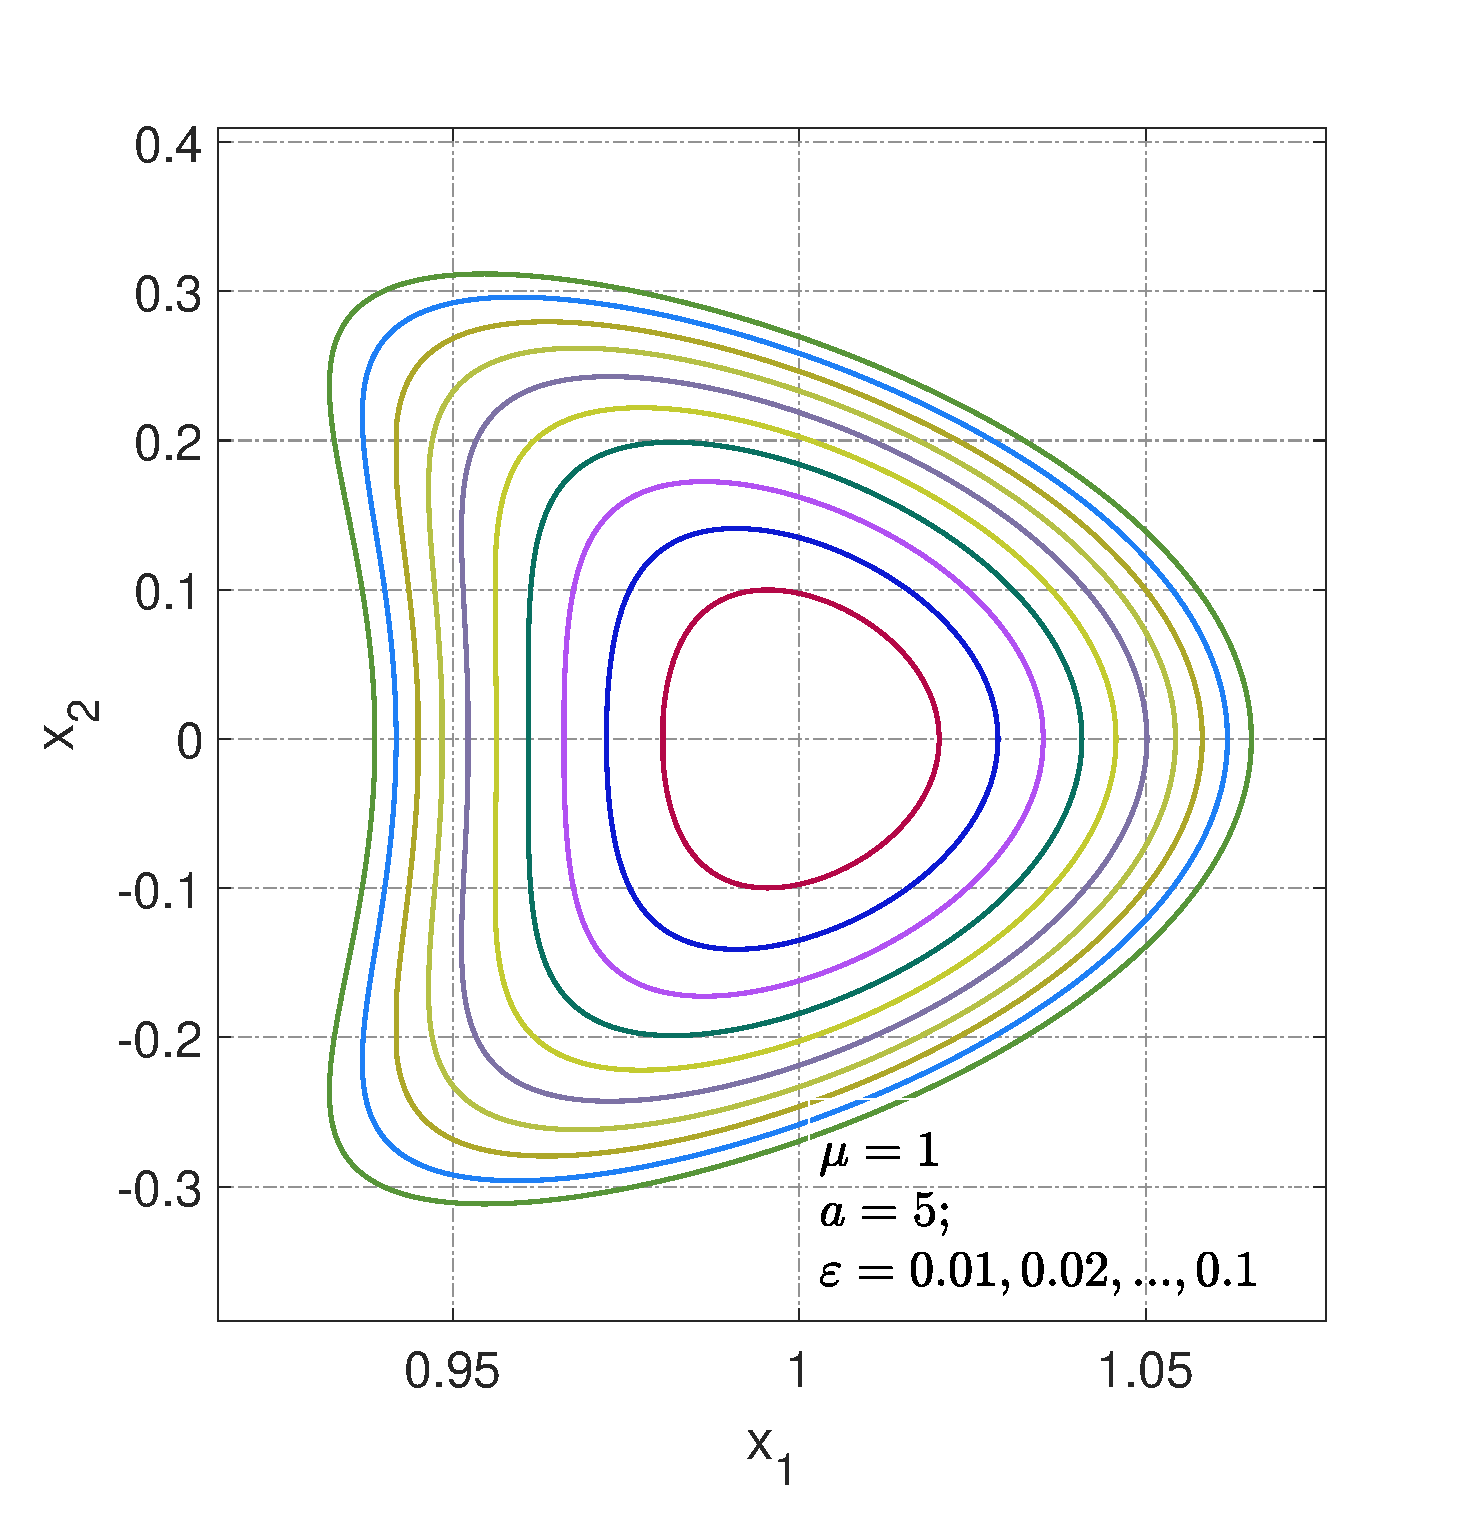
\includegraphics[width=1.05\linewidth]{images/figb11.eps}}
     \end{minipage}
     \hfill
     \begin{minipage}[h]{0.5\linewidth}
         \center{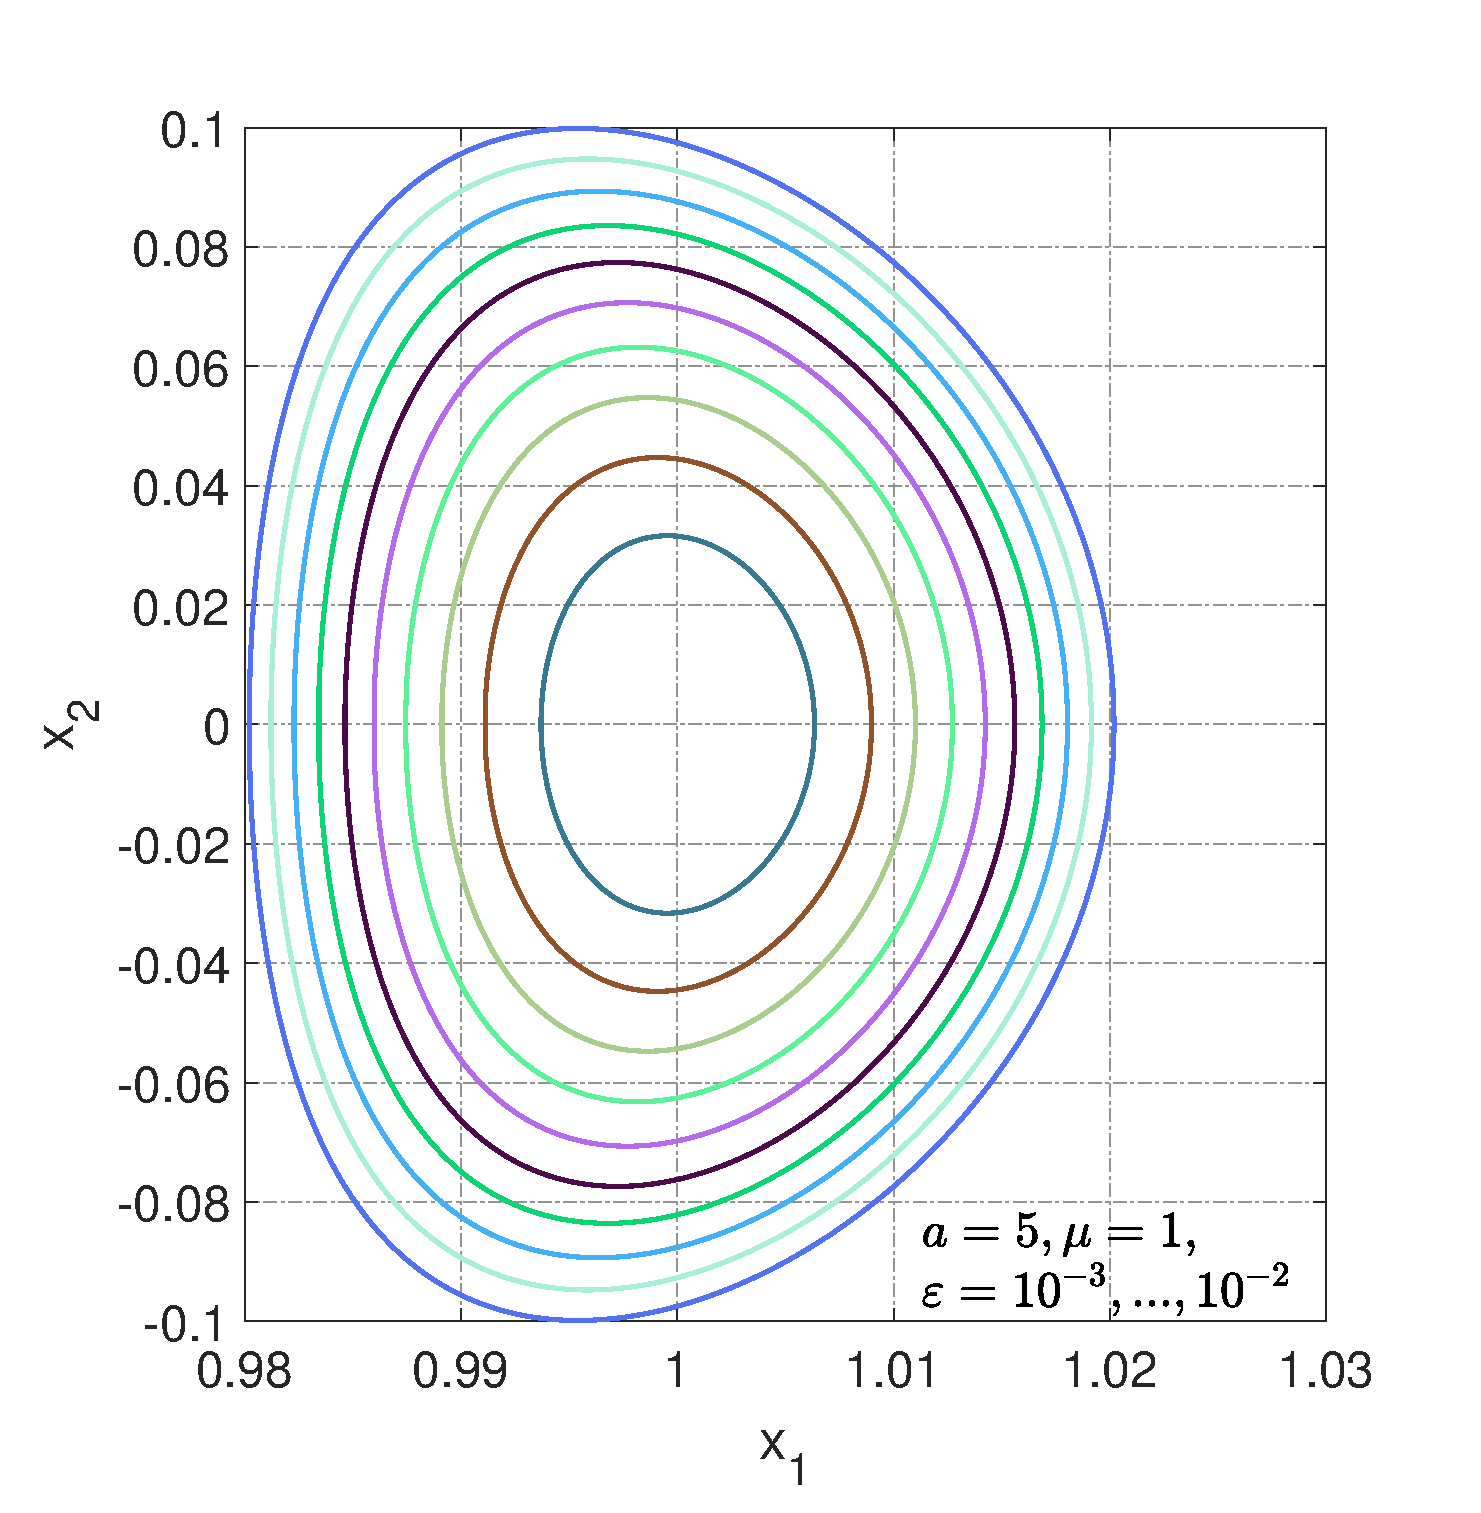
\includegraphics[width=1.05\linewidth]{images/figb21.eps}}
     \end{minipage}
     \caption{Множества достижимости билинейной системы}
     \label{sec1:fig:fig31}
\end{figure}
 
Для описания области достижимости системы \eqref{sec1:brokett} введем вспомогательную линейную систему
\begin{gather}\label{sec1:linearized_systembrokett}
     \left[ {\begin{array}{*{20}{c}}
             {{{\dot y}_1}}\\
             {{{\dot y}_2}}
     \end{array}} \right] = \left[ {\begin{array}{*{20}{c}}
             0&{ - 1}\\
             1&0
     \end{array}} \right]\left[ {\begin{array}{*{20}{c}}
             {{u_1}}\\
             {{u_2}}
     \end{array}} \right],
\end{gather}
множество достижимости которой является эллипсом $ G(t_1) = \left\lbrace y | y^T \left( B B^T\right)  ^{-1} y \leq \mu^2 \right\rbrace  $, где 
\begin{gather*}
     B = \left[ {\begin{array}{*{20}{c}}
             0&{ - 1}\\
             1&0
     \end{array}} \right].
\end{gather*}
 
Таким образом, множество достижимости системы \eqref{sec1:brokett} может быть получено путем нелинейного преобразования множества достижимости $ G(t_1) $ линейной системы \eqref{sec1:linearized_systembrokett}.
На рисунке  \ref{sec1:fig:fig31} показаны множества достижимости для различных $ \varepsilon $.
 
\begin{gather*}
\begin{array}{l}
         r({t_1}) = {e^{ \frac{1}{a} y_1}}\\
         \varphi ({t_1}) =  y_2. 
\end{array}
\end{gather*}
 % ссылка на тарасьева
\paragraph{Машина Дубинса.} 
Рассмотрим систему 
\begin{gather}\label{sec1:system6}
\begin{array}{*{20}{c}}
    {\left\{ {\begin{array}{*{20}{l}}
                     {{{\dot x}_1} = \cos {x_3}}\\
                     {{{\dot x}_2} = \sin {x_3}}\\
                     {{{\dot x}_3} = u}
\end{array}} \right.}&{{x_1}\left( 0 \right) = {x_2}\left( 0 \right) = {x_3}\left( 0 \right) = 0}
\end{array}
\end{gather}
на отрезке $ \left[0;\varepsilon \right] $, где $ \varepsilon > 0 $.
Ограничения на $ u\left(t \right) $ заданы неравенством 
\begin{gather}\label{sec1:constraints*}
    \int_{0}^{\vartheta} u^2(\tau) d\tau \leqslant \mu^2.
\end{gather}
 
При $  u_1(t) \equiv 0 $ получаем траекторию $ x_1(t) = t, \ x_2(t) = x_3(t) \equiv 0 $.
Как и в предыдущем примере, линеаризуем систему вдоль траектории, порожденной нулевым управлением
\begin{gather}\label{sec1:system6l}
     \left[ {\begin{array}{*{20}{c}}
             {{{\dot x}_1}}\\
             {{{\dot x}_2}}\\
             {{{\dot x}_3}}
     \end{array}} \right] = \varepsilon \underbrace {\left[ {\begin{array}{*{20}{c}}
                 0&0&0\\
                 0&0&1\\
                 0&0&0
         \end{array}} \right]}_A\left[ {\begin{array}{*{20}{c}}
             {{x_1}}\\
             {{x_2}}
     \end{array}} \right] + \underbrace {\left[ {\begin{array}{*{20}{c}}
                 0\\
                 0\\
                 1
         \end{array}} \right]}_Bu ,
\end{gather}
\begin{figure}[h]
     \centering
     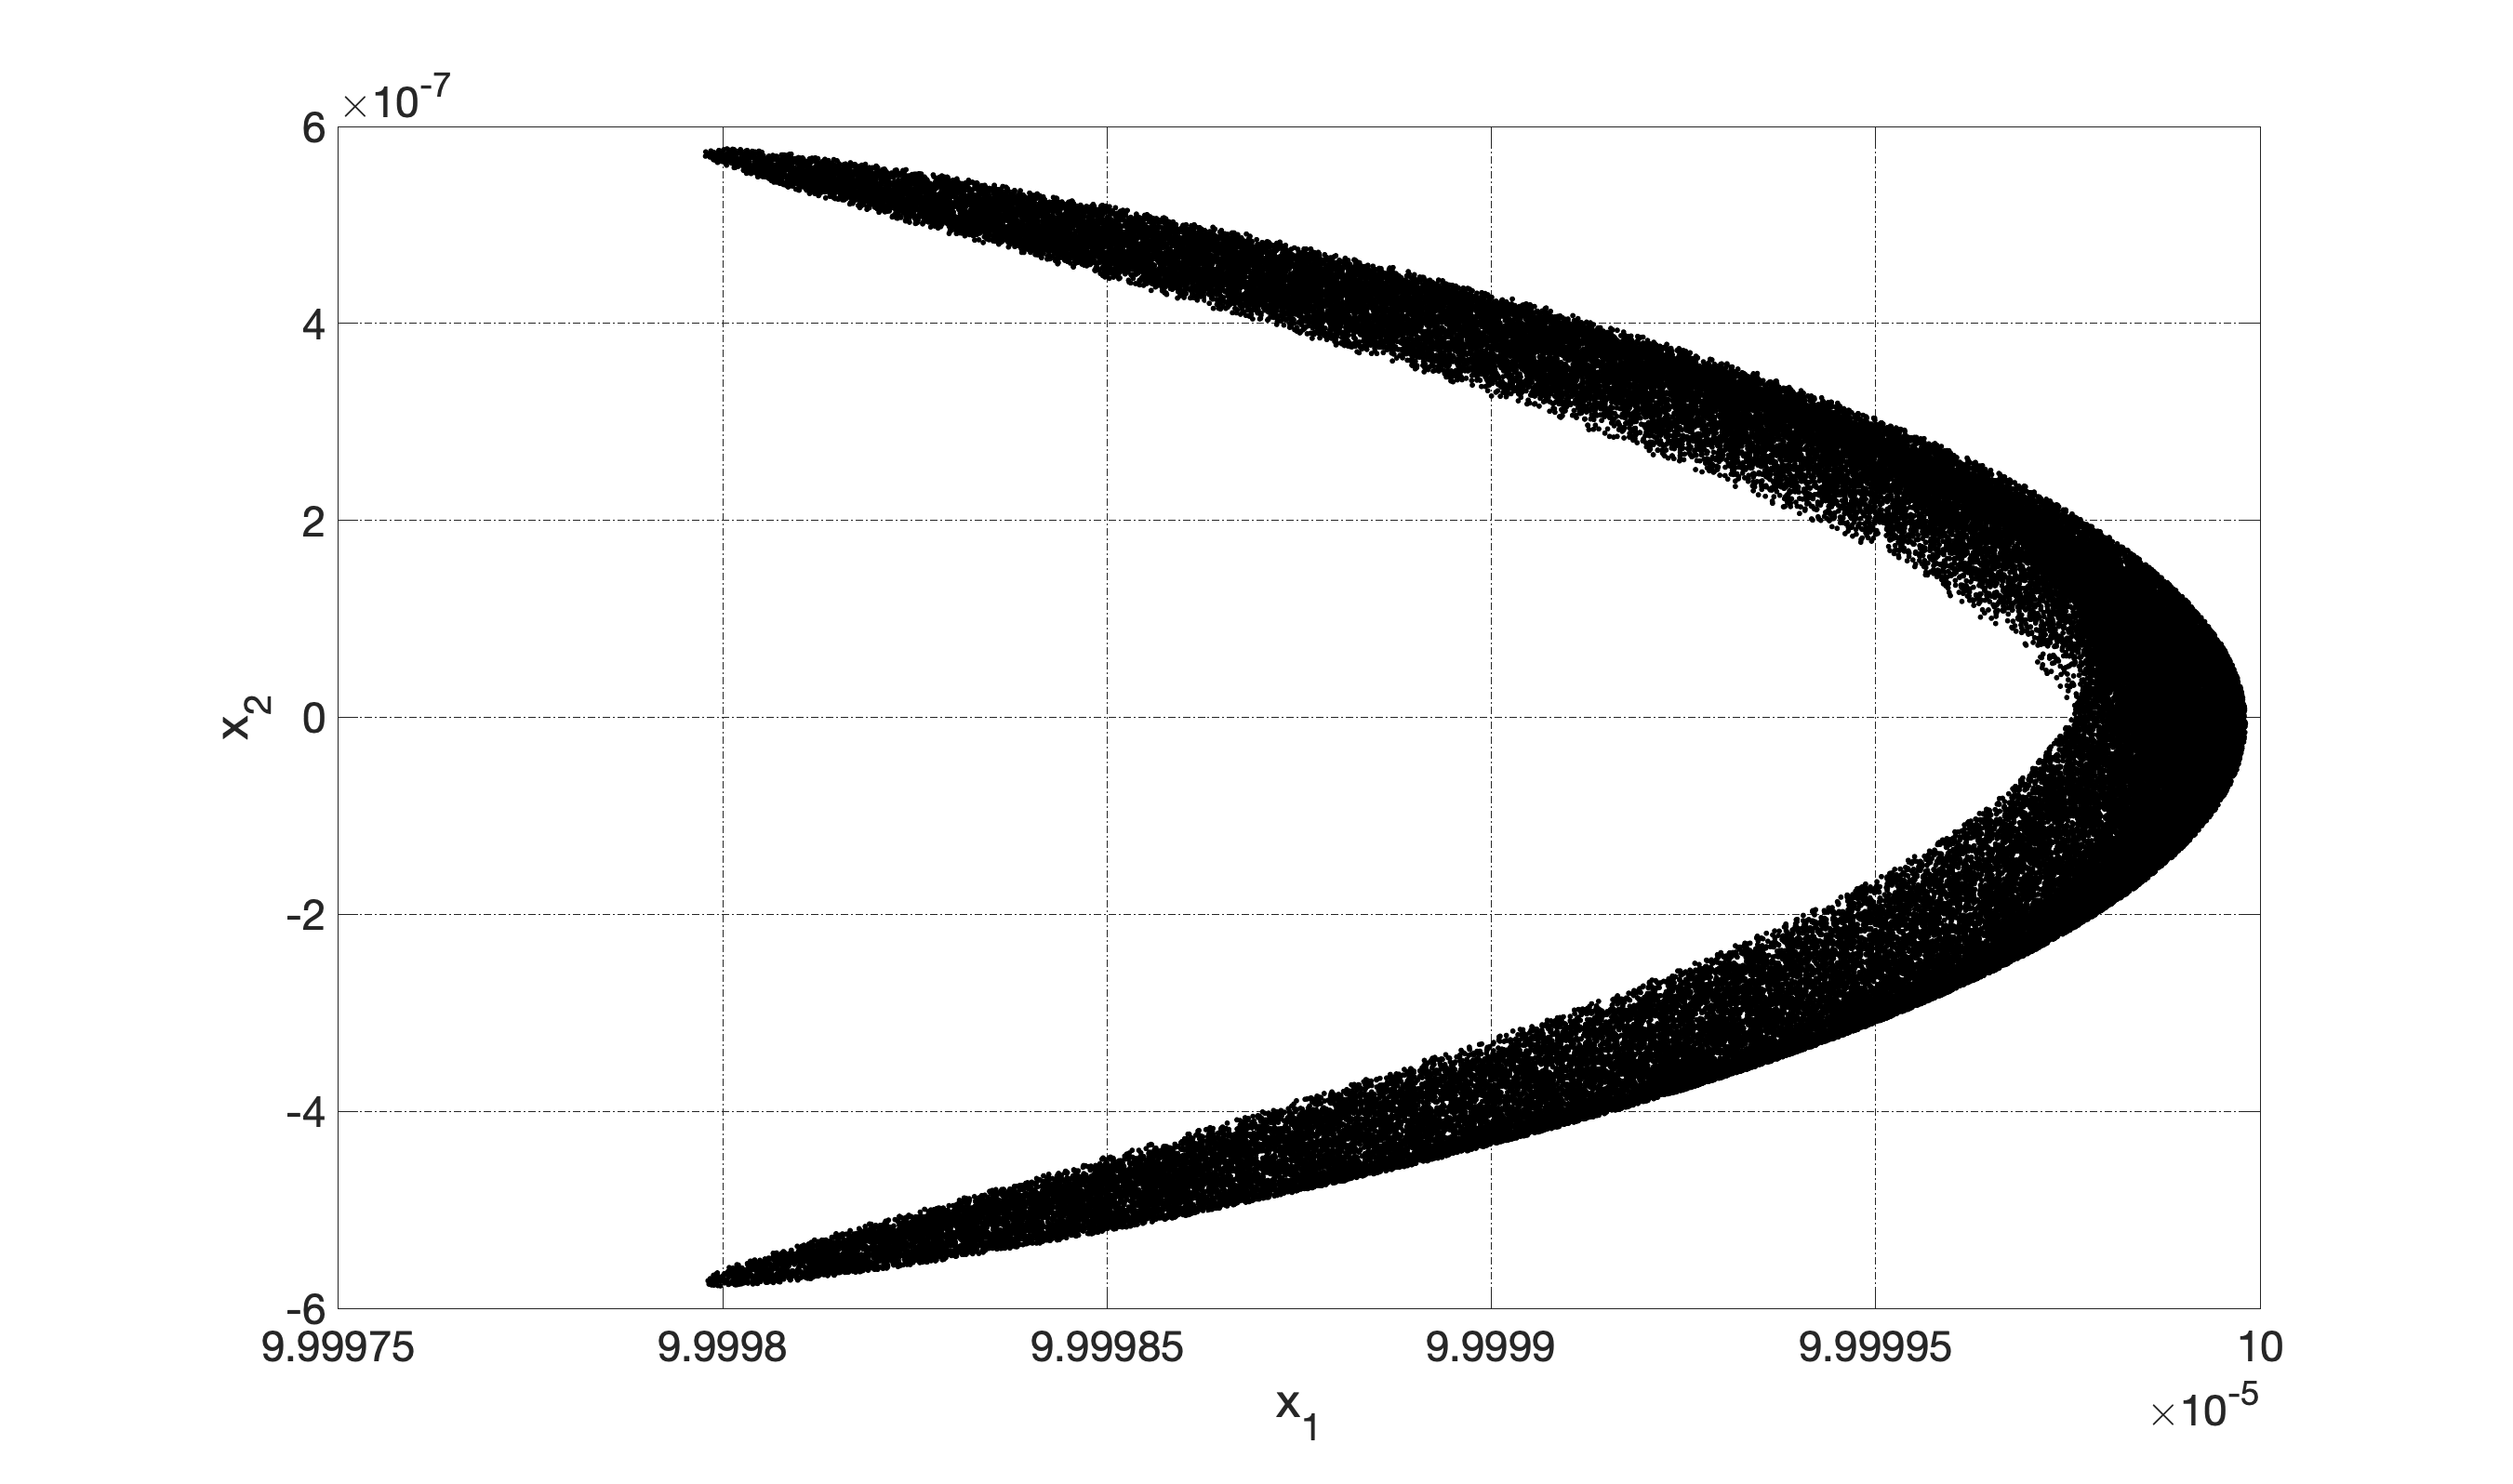
\includegraphics[width=1\linewidth]{images/fig52.eps}
     \caption{Множество достижимости машины Дубинса для $\varepsilon = 10^{-4}, \mu = 1$.}
     \label{sec1:fig:fig3}
\end{figure}
Очевидно, что система \eqref{sec1:system6l} неуправляема по 1-ой координате, следовательно, ее граммиан управляемости содержит нулевое собственное число, из-за которого условие \eqref{sec1:small_time_convexity_condition} не выполняется.
Следовательно, система \eqref{sec1:system6} может иметь невыпуклые множества достижимости на малых промежутках времени.
 
Воспользовавшись численным алгоритмом построения множеств достижимости систем с интегральными ограничениями \cite{GusevZykov2018} построим множество достижимости \eqref{sec1:system6} для $ \mu = 1  $ и $ \varepsilon = 0.0001  $ c. 
 
Моделирование показывает, что множество достижимости <<машины Дубинса>> невыпукло для достаточно малых $ \varepsilon $; это можно показать и теоретически, но строгое доказательство невыпуклости выходит за рамки этого раздела.
 
\end{document}